\documentclass[a4paper,12pt,twoside,openany]{report}
%
% Wzorzec pracy dyplomowej
% J. Starzynski (jstar@iem.pw.edu.pl) na podstawie pracy dyplomowej
% mgr. inż. Błażeja Wincenciaka
% Wersja 0.1 - 8 października 2016
%
\usepackage{polski}
\usepackage{helvet}
\usepackage[T1]{fontenc}
\usepackage{anyfontsize}
\usepackage[utf8]{inputenc}
\usepackage[pdftex]{graphicx}
\usepackage{tabularx}
\usepackage{array}
\usepackage[polish]{babel}
\usepackage{subfigure}
\usepackage{amsfonts}
\usepackage{verbatim}
\usepackage{indentfirst}
\usepackage[pdftex]{hyperref}


% rozmaite polecenia pomocnicze
% gdzie rysunki?
\newcommand{\ImgPath}{.}

% oznaczenie rzeczy do zrobienia/poprawienia
\newcommand{\TODO}{\textbf{TODO}}


% wyroznienie slow kluczowych
\newcommand{\tech}{\texttt}

% na oprawe (1.0cm - 0.7cm)*2 = 0.6cm
% na oprawe (1.1cm - 0.7cm)*2 = 0.8cm
%  oddsidemargin lewy margines na nieparzystych stronach
% evensidemargin lewy margines na parzystych stronach
\def\oprawa{1.05cm}
\addtolength{\oddsidemargin}{\oprawa}
\addtolength{\evensidemargin}{-\oprawa}

% table span multirows
\usepackage{multirow}
\usepackage{enumitem}	% enumitem.pdf
\setlist{listparindent=\parindent, parsep=\parskip} % potrzebuje enumitem

%%%%%%%%%%%%%%% [nazarewk] Z templatki pandoc %%%%%%%%%%%%%%%%
\providecommand{\tightlist}{%
  \setlength{\itemsep}{0pt}\setlength{\parskip}{0pt}}


% For code highlighting


\usepackage{listings}
\newcommand{\passthrough}[1]{#1}
\usepackage{xcolor}

\usepackage{listingsutf8}
\usepackage[ttdefault=true]{AnonymousPro}
\lstset{
    basicstyle=\fontsize{9}{11}\ttfamily,
    keywordstyle=\color[rgb]{0.13,0.29,0.53}\bfseries,
    stringstyle=\color[rgb]{0.31,0.60,0.02},
    commentstyle=\color[rgb]{0.56,0.35,0.01}\itshape,
    numberstyle=\footnotesize,
    stepnumber=1,
    numbersep=5pt,
    backgroundcolor=\color[RGB]{248,248,248},
    showspaces=false,
    showstringspaces=false,
    showtabs=false,
    tabsize=2,
    captionpos=b,
    breaklines=true,
    breakatwhitespace=false,
    breakautoindent=true,
    escapeinside={\%*}{*)},
    linewidth=\textwidth,
    basewidth=0.6em,
    rulecolor=\color{black},
    inputencoding=utf8,
    frame=single,
}
\lstset{postbreak=\raisebox{0ex}[0ex][0ex]{\ensuremath{\color{red}\hookrightarrow\space}}}

\raggedbottom

% Przypisy na końcu dokumentu
\renewcommand{\href}[2]{#2\endnote{\url{#1}}}
\usepackage{endnotes}
\usepackage{hyperendnotes}
\renewcommand{\thefootnote}{\fnsymbol{footnote}}
% Wyczyść nagłówek (wykorzystamy nagłówek z markdowna)
\def\enoteheading{}

%%%%%%%%%%%%%%% Dodatkowe Pakiety %%%%%%%%%%%%%%%%%
\usepackage{prmag2017}   % definiuje komendy opieku,nrindeksu, rodzaj pracy, ...


%%%%%%%%%%%%%%% Strona Tytułowa %%%%%%%%%%%%%%%%%
% To trzeba wypelnic swoimi danymi
\title{Implementacja i testy wydajności środowiska Kubernetes na maszynach bezdyskowych}

% autor
\author{Krzysztof Nazarewski}
\nrindeksu{240579}

\opiekun{mgr inż. Andrzej Toboła}
%\konsultant{prof. Dzielny Konsultant}  % opcjonalnie
\terminwykonania{7 lutego 2018} % data na oświadczeniu o samodzielności
\rok{2018}


% Podziekowanie - opcjonalne
\podziekowania{%\noindent
%{\Large Podziękowania}
%\bigskip
%
%Dziękujemy bardzo serdecznie wszystkim, a w szczególności Rodzinom i~Unii Europejskiej...
%
%\bigskip
%
%{\raggedleft
%Zdolny Student i Pracowity Kolega
%
%}
%
}

% To sa domyslne wartosci
% - mozna je zmienic, jesli praca jest pisana gdzie indziej niz w ZETiIS
% - mozna je wyrzucic jesli praca jest pisana w ZETiIS
%\miasto{Warszawa}
%\uczelnia{POLITECHNIKA WARSZAWSKA}
%\wydzial{WYDZIAŁ ELEKTRYCZNY}
%\instytut{INSTYTUT ELEKTROTECHNIKI TEORETYCZNEJ\linebreak[1] I~SYSTEMÓW INFORMACYJNO-POMIAROWYCH}
% \zaklad{ZAKŁAD ELEKTROTECHNIKI TEORETYCZNEJ\linebreak[1] I~INFORMATYKI STOSOWANEJ}
%\kierunekstudiow{INFORMATYKA}

% domyslnie praca jest inzynierska, ale po odkomentowaniu ponizszej linii zrobi sie magisterska
%\pracamagisterska
%%% koniec od P.W

\opinie{%
  \input{opiniaopiekuna.tex}
  \newpage
  \input{recenzja.tex}
}

\streszczenia{
  \newpage
\begin{center}
  \large \bf
  Implementacja środowiska Kubernetes na maszynach bezdyskowych
\end{center}

\section*{Streszczenie}

Celem tej pracy inżynierskiej jest przybliżenie czytelnikowi zagadnień
związanych z systemem Kubernetes oraz jego uruchamianiem na maszynach
bezdyskowych.

Zacznę od wyjaśnienia pojęcia kontenerów, problemu orkiestracji nimi i krótkiego
teoretycznego przeglądu dostępnych rozwiązań.
Opiszę czym jest Kubernetes, jaką ma architekturę oraz przedstawię podstawowe
pojęcia pozwalające na zrozumienie i korzystanie z niego.
Opis Kubernetes zakończę przedstawieniem sposobów jego uruchomienia na maszynach
bezdyskowych.

Następnie przeprowadzę krótki teoretyczno-praktyczny przegląd systemów
operacyjnych i sposobów uruchamiania Kubernetes na nich.

Po ich wybraniu przeprowadzę testy na sieci uczelnianej, a na koniec doprowadzę
ją do stanu docelowego pozwalającego na przeprowadzenie laboratoriów Kubernetes.

\bigskip
{\noindent\bf Słowa kluczowe:} Kubernetes, konteneryzacja, orkiestracja, maszyny bezdyskowe

\vskip 2cm


\begin{center}
  \large \bf
  Implementing Kubernetes on diskless machines
\end{center}

\section*{Abstract}

Primary goal of this document is to present basic concepts related to Kuberentes
and running it on diskless systems.

I will start with explaining what are containers, problem of their orchestration
and I will theoretically inspect available solutions.

I will describe what is Kuberentes, provide overview of it's architecture and
basic concepts allowing to understand and use it.
I will end the description with overview of it's provisioning tools working on
diskless systems.

Then I will research and conduct brief practical tests of available operating
systems and provisioning tools.

After selecting solutions I will conduct practical tests on university network
and finally configure Kubernetes to run the network.

\bigskip
{\noindent\bf Keywords:} Kubernetes, containerization, orchestration, diskless systems

\vfill
}

\begin{document}
\maketitle
\hypertarget{wstux119p}{%
\chapter{Wstęp}\label{wstux119p}}

Historia wirtualizacji i przydzielania zasobów sięga już pierwszych
systemów komputerowych.

Podstawową przeszkodą w korzystaniu z komputerów była ich wysoka cena;
bogate instytucje odpłatnie wynajmowały swoje systemy innym firmom.
Umożliwiając dostęp tylko jednemu użytkownikowi jednocześnie, maszyny
przez większość czasu nie pracowały. Wraz ze wzrostem liczby
obsługiwanych użytkowników przypadających na jedną maszynę~zwiększało
się wysycenie jej zasobów, a zatem i zyski.

Następną przeszkodą okazał się brak ograniczeń dostępowych dla
poszczególnych użytkowników: każdy świadomie lub nie mógł uszkodzić
cudze zasoby. W ten sposób zrodził się pomysł
\passthrough{\lstinline!chroot!}, czyli izolacji użytkowników na
poziomie systemu plików.

Wraz z rozwojem technologii zwiększała się różnorodność sprzętowa i
systemowa. W związku z pierwszą systemy operacyjne oferowały abstrakcje
dostępu do sprzętu oraz powstawały narzędzia emulujące inny sprzęt.
Różnorodność systemowa była natomiast abstrahowana przez aplikacyjne
wirtualne maszyny, które umożliwiały jednorodny dostęp do zasobów
niejednorodnych systemów operacyjnych, ale w żaden sposób go nie
ograniczały.

W centrach danych zyskała popularność~wirtualizacja sprzętowa. Pozwala
ona uruchomić na jednej fizycznej maszynie wiele niezależnych od siebie
maszyn wirtualnych, na których działają dowolne systemy operacyjne. W
toku rozwoju technologii po roku 2000 pojawił się trend rozpraszania
oprogramowania i dążenia do uruchamiania jak najmniejszej jego
funkcjonalnej części na pojedynczej maszynie wirtualnej. Główną~zaletą
takiego podejścia jest bezpieczeństwo: po uzyskaniu dostępu do jednego z
serwerów włamywacz nadal nie ma dostępu do reszty infrastruktury.
Wadą~natomiast jest to, że jedna maszyna fizyczna jest w stanie
uruchomić nie więcej niż~kilka do kilkunastu maszyn wirtualnych. W
związku z tym utrzymywanie całej maszyny wirtualnej w celu uruchamiania
pojedynczego procesu aplikacyjnego często jest nieekonomiczne.

Na przełomie ostatniej dekady zaczęły pojawiać się narzędzia pozwalające
uruchamiać wiele w pełni odizolowanych procesów współdzielących jedynie
jądro systemu operacyjnego. Znacznie zmniejszyło to narzut zasobów
wymaganych do uruchamiania kolejnych aplikacji-procesów i umożliwiło
współdzielenie jednej maszyny przez setki, a nawet tysiące programów.
Metodologia ta zyskała miano konteneryzacji i jest z powodzeniem
wykorzystywana w systemach produkcyjnych na całym świecie.

Technologia konteneryzacji jest młoda, a konkurencja duża. Z jednej
strony trwa wyścig o stworzenie najlepszego rozwiązania, a z drugiej
aktywnie rozwijane są~ otwarte standardy konteneryzacji w ramach
\href{https://www.opencontainers.org/about}{\passthrough{\lstinline!Open Container Initiative!}},
ponieważ nikt nie może pozwolić sobie na niekompatybilność swojej
implementacji. Obecnie najpopularniejszą implementacją kontenerów jest
\passthrough{\lstinline!Docker!}.

Aspektem równie ważnym jak sama implementacja kontenerów, jest kwestia
zarządzania nimi. O ile kilkoma serwerami z kilkudziesięcioma
kontenerami może zarządzać człowiek, o tyle do zarządzania tysiącami
kontenerów wymagany jest w dużej mierze zautomatyzowany i
wyspecjalizowany system.

Obecnie przodującym rozwiązaniem tego problemu jest
\passthrough{\lstinline!Kubernetes!} (zamiennie
\passthrough{\lstinline!k8s!}). Projekt powstał niedawno (w połowie 2014
roku) i mimo tego, że coraz bardziej umacnia swoją pozycję~na rynku
nadal umie go skonfigurować tylko nieliczne grono specjalistów. Celem
niniejszej pracy jest przedstawienie sposobu konfiguracji klastra
\passthrough{\lstinline!k8s!} na fizycznych maszynach\footnote{ang.
  \emph{bare metal}, czyli uruchamianie na prostej sieci komputerowej
  bez zewnętrznych zależności, w odróżnieniu od kompleksowych usług
  chmurowych, które w znacznym stopniu automatyzują~i ułatwiają
  konfigurację} na przykładzie sieci komputerowej Wydziału Elektrycznego
Politechniki Warszawskiej. Laboratoria komputerowe dostępne w tej sieci
są wyposażone w maszyny bezdyskowe, a zatem należy pokrótce
scharakteryzować tego typu systemy.

\hypertarget{charakterystyka-systemuxf3w-bezdyskowych}{%
\section{Charakterystyka systemów
bezdyskowych}\label{charakterystyka-systemuxf3w-bezdyskowych}}

W dzisiejszych czasach rozwój sieci komputerowych i spadek cen pamięci
RAM pozwolił na konfigurację maszyn nie posiadających dysku twardego.
Bezdyskowe maszyny przy starcie pytają centralny serwer o swoją
konfigurację (np. protokołem \passthrough{\lstinline!PXE!}), a następnie
umieszczają kompletny system operacyjny w pamięci RAM.

W momencie wyłączenia maszyny cały stan jest tracony, a przy ponownym
rozruchu konfigurowana jest od nowa. w celu trwałego przechowywania
danych systemy bezdyskowe korzystają z zewnętrznych serwerów plikowych.

Rozwiązanie pozwala to na jednorazową konfigurację~bazowego systemu
operacyjnego i uzyskanie konfiguracji na dowolnej ilości maszyn bez
ingerencji człowieka. W efekcie koszt utrzymania centrów danych przenosi
się z konfiguracji indywidualnych maszyn na konfigurację pojedynczych
usług działających na dowolnej liczbie maszyn.

Zarządzanie klastrem \passthrough{\lstinline!k8s!} poza środowiskiem
chmurowym znacznie ogranicza wybór narzędzia konfiguracyjnego, a
bezdyskowość jego węzłów ma duży wpływ na wybór systemu operacyjnego.

\hypertarget{system-kubernetes}{%
\chapter{System Kubernetes}\label{system-kubernetes}}

\href{https://kubernetes.io/}{\passthrough{\lstinline!Kubernetes!}}
został stworzony przez firmę Google na bazie ich wewnętrznego systemu
\passthrough{\lstinline!Borg!}, a następnie udostępniony na zasadach
otwartego oprogramowania (ang. \emph{open-source}). Charakteryzuje się
korzystnym stosunkiem kosztów zarządzania do oferowanych możliwości.

\hypertarget{pod}{%
\paragraph{\texorpdfstring{\texttt{Pod}}{Pod}}\label{pod}}

jest podstawową~i niepodzielną jednostką~aplikacyjną klastra
\passthrough{\lstinline!k8s!} dalej zwaną instancją~aplikacji~lub po
prostu instancją. W rozdziale ``Podstawowe rodzaje obiektów
aplikacyjnych'' znajdują się bardziej szczegółowe informacje dotyczące
tego zagadnienia.

\hypertarget{kontroler}{%
\paragraph{Kontroler}\label{kontroler}}

jest ogólnym określeniem grupy obiektów zarządzających instancjami
aplikacji.

\hypertarget{zarzux105dzanie-klastrem}{%
\paragraph{Zarządzanie klastrem}\label{zarzux105dzanie-klastrem}}

rozumiem jako zbiór czynności i procesów polegających na przygotowaniu
klastra do użytku oraz definiowanie aplikacji realizującymi usługi na
poziomie klastra, takimi jak:

\begin{itemize}
\tightlist
\item
  tworzenie klastra,
\item
  dodawanie i usuwanie fizycznych węzłów,
\item
  integracja z sieciowym systemem plikowym,
\item
  integracja z zewnętrznymi systemami zarządzania kontami użytkowników,
\item
  nadawanie uprawnień użytkownikom i procesom,
\item
  centralny system zbierania dzienników aplikacji (ang.
  \emph{centrallized logging system}),
\item
  centralny system monitorujący obciążenie węzłów,
\end{itemize}

\hypertarget{wykorzystanie-klastra}{%
\paragraph{Wykorzystanie klastra}\label{wykorzystanie-klastra}}

rozumiem jako uruchamianie dowolnych aplikacji na wcześniej
skonfigurowanym klastrze.

\hypertarget{stan-w-klastrze-kubernetes}{%
\paragraph{Stan w klastrze
Kubernetes}\label{stan-w-klastrze-kubernetes}}

zdefiniowany jest jako konfiguracja, do której klaster dąży.

\hypertarget{status-w-klastrze-kubernetes}{%
\paragraph{Status w klastrze
Kubernetes}\label{status-w-klastrze-kubernetes}}

zdefiniowany jest jako rzeczywista konfiguracja, w której klaster się w
danej chwili znajduje.

Zwykle stan i status klastra szybko się ze sobą~zbiegają, ale nie jest
to regułą. Dwoma najczęstszymi powodami braku ich synchronizacji
są~niewystarczające zasoby lub utrata węzła roboczego.

W pierwszym przypadku stan klastra może wskazywać na istnienie 5
instancji aplikacji, ale pamięci RAM wystarcza na uruchomienie tylko 3.
Więc bez zmiany infrastruktury brakujące 2 instancje nigdy nie zostaną
uruchomione. W momencie dołączenia kolejnego węzła klastra może się
okazać, że posiadamy już wymagane zasoby i aplikacja zostanie
uruchomiona w pełni, czyli stan aplikacji pokryje się z jej statusem.

W drugim przypadku mając działające 4 instancje aplikacji na 2 węzłach,
po utraceniu drugiego węzła stan kontrolera będzie nadal wskazywał na 4
instancje, a status na 2. W ciągu kilku do kilkudziesięciu sekund
kontroler zauważy braki, uruchomi brakujące 2 instancje na pierwszym
węźle i przez to doprowadzi status klastra do stanu docelowego.

\hypertarget{struktura-klastra-kubernetes}{%
\section{Struktura klastra
Kubernetes}\label{struktura-klastra-kubernetes}}

Wysokopoziomową~strukturę~klastra \passthrough{\lstinline!k8s!}
przedstawia poniższy schemat:

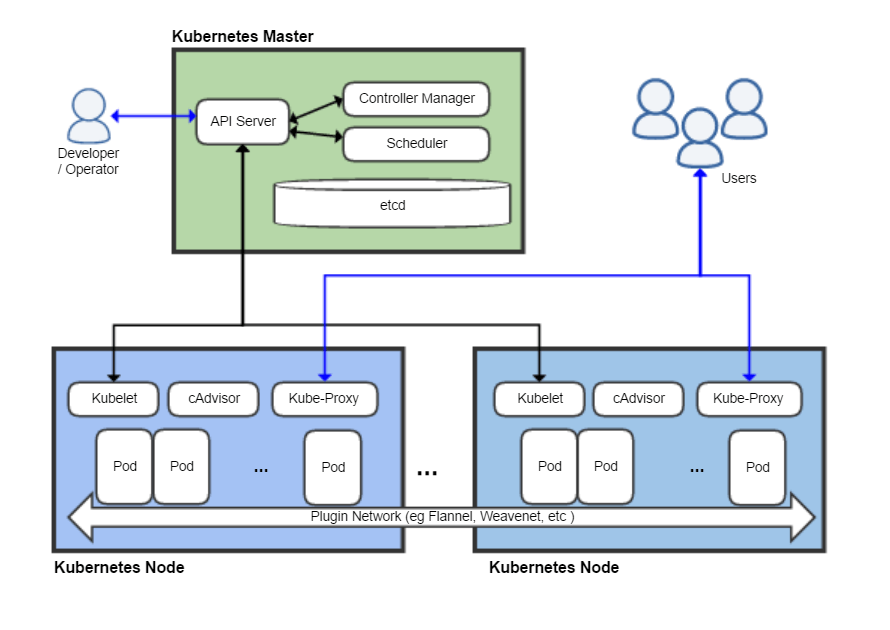
\includegraphics[width=5.20833in,height=3.6875in]{assets/kubernetes-architecture.png}\\

Na ilustracji wyróżnione zostało 5 grup funkcjonalnych:

\begin{enumerate}
\def\labelenumi{\arabic{enumi}.}
\tightlist
\item
  administrator lub programista korzystający z klastra -
  \passthrough{\lstinline!Developer/Operator!},
\item
  użytkowników końcowi aplikacji działających w klastrze -
  \passthrough{\lstinline!Users!},
\item
  jeden lub więcej węzeł zarządzający -
  \passthrough{\lstinline!Kubernetes Master!},
\item
  jeden lub więcej węzeł roboczy -
  \passthrough{\lstinline!Kubernetes Node!},
\item
  wtyczka sieciowa (\passthrough{\lstinline!Plugin Network!}), czyli
  oprogramowanie realizujące komunikację sieciową w ramach klastra
  \passthrough{\lstinline!k8s!}.
\end{enumerate}

\hypertarget{pux142aszczyzna-zarzux105dzajux105ca}{%
\subsubsection{Płaszczyzna
zarządzająca}\label{pux142aszczyzna-zarzux105dzajux105ca}}

Węzeł~zarządzający zilustrowany został jako jedna maszyna, ale w trybie
wysokiej dostępności składa się z co najmniej trzech kopii. W związku z
tym trafniejszą jego nazwą jest ``płaszczyzna zarządzająca'' (ang.
\emph{Control Plane}).

\hypertarget{etcd}{%
\paragraph{\texorpdfstring{\texttt{etcd}}{etcd}}\label{etcd}}

jest bazą danych kluczy i wartości, w której przechowywany jest zarówno
stan, jak i status klastra. Jest koncepcyjnie proste, żeby ułatwić
skupienie się na jej wydajności, stabilności i skalowaniu. Mimo że
najczęściej przedstawia się je jako składową węzła zarządzającego, nie
jest to regułą, a tym bardziej wymogiem.

\hypertarget{kube-apiserver}{%
\paragraph{\texorpdfstring{\texttt{kube-apiserver}}{kube-apiserver}}\label{kube-apiserver}}

jest jedynym sposobem na interakcję z \passthrough{\lstinline!etcd!} w
ramach klastra \passthrough{\lstinline!k8s!}. Zarówno zewnętrzni
użytkownicy, jak i wewnętrzne procesy klastra korzystają z interfejsu
aplikacyjnego REST (ang. REST API) oferowanego przez
\passthrough{\lstinline!kube-apiserver!} w celu uzyskania informacji i
zmiany jego stanu.

\hypertarget{kube-controller-manager}{%
\paragraph{\texorpdfstring{\texttt{kube-controller-manager}}{kube-controller-manager}}\label{kube-controller-manager}}

jest głównym modułem zarządzającym, który dba o doprowadzenia klastra do
oczekiwanego stanu. Uruchamia on pętlę kontrolującą klaster, na której
bazuje wiele procesów kontrolnych, jak na przykład kontroler replikacji
i kontroler kont serwisowych.

\hypertarget{kube-scheduler}{%
\paragraph{\texorpdfstring{\texttt{kube-scheduler}}{kube-scheduler}}\label{kube-scheduler}}

jest modułem zarządzającym zasobami klastra. Decyduje on, na których
węzłach uruchamiać aplikacje, żeby zaspokoić popyt na zasoby,
jednocześnie nie przeciążając pojedynczych węzłów klastra.

\hypertarget{wux119zeux142-roboczy}{%
\subsubsection{Węzeł roboczy}\label{wux119zeux142-roboczy}}

W klastrze \passthrough{\lstinline!k8s!} istnieją tylko dwa niezbędne
elementy węzła roboczego, ale w praktyce każdy z węzłów ma uruchomiony
cały wachlarz aplikacji ułatwiających zarządzanie nimi. Zilustrowanym
przykładem jest \passthrough{\lstinline!cAdvisor!}.

\hypertarget{kubelet}{%
\paragraph{\texorpdfstring{\texttt{kubelet}}{kubelet}}\label{kubelet}}

jest podstawowym procesem działającym na węzłach roboczych. Monitoruje i
kontroluje kontenery działające w ramach jednego węzła. Na przykład
wiedząc, że na węźle mają działać 2 instancje aplikacji dba o to, żeby
restartować instancje działające nieprawidłowo, dodawać~nowe lub
wyłączać nadwyżkowe.

\hypertarget{kube-proxy}{%
\paragraph{\texorpdfstring{\texttt{kube-proxy}}{kube-proxy}}\label{kube-proxy}}

jest drugim najważniejszym procesem węzła roboczego odpowiadającym za
przekierowywanie ruchu sieciowego do odpowiednich kontenerów w ramach
klastra.

\hypertarget{cadvisor}{%
\paragraph{\texorpdfstring{\texttt{cAdvisor}}{cAdvisor}}\label{cadvisor}}

jest opcjonalnym elementem węzła roboczego, który monitoruje zużycie
zasobów i wydajność kontenerów w ramach jednego klastra. Umożliwia
automatyczne skalowanie aplikacji, na przykład na podstawie dużego
obciążenia pamięci RAM lub procesora.

\hypertarget{komunikacja-sieciowa}{%
\subsubsection{Komunikacja sieciowa}\label{komunikacja-sieciowa}}

Podstawowym założeniem \passthrough{\lstinline!k8s!} jest posiadanie
własnego adresu IP przez każdą aplikację działającą w klastrze, ale
nienarzucanie rozwiązania je realizującego to założenie. Administrator
klastra musi zadbać o konfigurację odpowiednich narzędzi, zwanych w
nomenklaturze \passthrough{\lstinline!k8s!} \emph{overlay network}.
Najprostsze koncepcyjnie jest stworzenie na każdym węźle wpisów
\passthrough{\lstinline!iptables!} przekierowujących adresy IP na
wszystkie inne węzły, a najpopularniejszymi rozwiązaniami są:
\href{https://github.com/coreos/flannel\#flannel}{\passthrough{\lstinline!Flannel!}}
i
\href{https://www.projectcalico.org/}{\passthrough{\lstinline!Project Calico!}}.

W klastrze \passthrough{\lstinline!k8s!} istnieją~4 podstawowe rodzaje
komunikacji sieciowej:

\begin{enumerate}
\def\labelenumi{\arabic{enumi}.}
\tightlist
\item
  wewnątrz kontenerów należących do jednej instancji na adresie
  \passthrough{\lstinline!127.0.0.1!},
\item
  pomiędzy instancjami w klastrze realizowana przez
  \passthrough{\lstinline!overlay network!},
\item
  między instancjami i serwisami realizowana przez
  \passthrough{\lstinline!kube-proxy!},
\item
  między serwisami, a światem realizowana serwisami typu
  \passthrough{\lstinline!LoadBalancer!} lub mechanizmem
  \passthrough{\lstinline!Ingress!},
\end{enumerate}

Poza nakładką~sieciową realizującą połączenie między kontenerami (w
ramach adresu \passthrough{\lstinline!127.0.0.1!}) składającymi się na
aplikację istnieją jeszcze komunikacja aplikacji z serwisami i serwisami
z siecią~zewnętrzną.

\hypertarget{serwis}{%
\paragraph{Serwis}\label{serwis}}

(ang. \passthrough{\lstinline!Service!}) jest podstawowym sposobem na
zautomatyzowanie komunikacji z instancjami aplikacji zarówno w obrębie
klastra jak i z poza niego. Podstawowymi rodzajami serwisów są:

\begin{itemize}
\tightlist
\item
  \passthrough{\lstinline!ClusterIP!} udostępniający instancję na
  wewnętrznym adresie IP,
\item
  \passthrough{\lstinline!NodePort!} udostępniający instancję na
  zewnętrznym adresie IP i porcie węzła na którym został uruchomiony,
\item
  \passthrough{\lstinline!LoadBalancer!} konfigurujący zewnętrzną
  usługę~przekierowującą zapytania do automatycznie tworzonego serwisu
  typu \passthrough{\lstinline!ClusterIP!} lub
  \passthrough{\lstinline!NodePort!},
\end{itemize}

\hypertarget{ingress}{%
\paragraph{\texorpdfstring{\texttt{Ingress}}{Ingress}}\label{ingress}}

jest mechanizmem umożliwiającym eksponowanie instancji poza klaster, tak
jak ma to miejsce w serwisie typu
\passthrough{\lstinline!LoadBalancer!}, ale dającym większe możliwości
konfiguracji, na przykład eliminując zależność od usług chmurowych.
Obecnie istnieją kontrolery \passthrough{\lstinline!Ingress!} bazujące
na serwerze
\href{https://github.com/kubernetes/ingress-nginx}{\passthrough{\lstinline!nginx!}}
i
\href{https://github.com/kubernetes/ingress-gce}{\passthrough{\lstinline!GCE!}}.

\hypertarget{zarzux105dzanie-dostux119pami}{%
\subsubsection{Zarządzanie
dostępami}\label{zarzux105dzanie-dostux119pami}}

Podstawowymi pojęciami związanymi z zarządzaniem dostępami w
\passthrough{\lstinline!k8s!} są uwierzytelnianie, autoryzacja i
przestrzenie nazw (obiekt \passthrough{\lstinline!Namespace!}).

\hypertarget{uwierzytelnianie}{%
\paragraph{Uwierzytelnianie}\label{uwierzytelnianie}}

jest pierwszym krokiem w każdym zapytaniu do API. Polega na weryfikacji,
że użytkownik (lub wewnętrzna aplikacja) jest tym za kogo się podaje.
Podstawowymi sposobami uwierzytelniania są:

\begin{itemize}
\tightlist
\item
  certyfikaty klienckie X509,
\item
  statyczne przepustki (ang. \emph{token}),
\item
  przepustki rozruchowe (ang. \emph{bootstrap tokens}),
\item
  statyczny plik z hasłami,
\item
  przepustki kont serwisowych (ang.
  \passthrough{\lstinline!ServiceAccount!} tokens),
\item
  przepustki OpenID Connect,
\item
  zapytanie uwierzytelniające do zewnętrznego serwisu (ang.
  \emph{webhook}),
\item
  proxy uwierzytelniające.
\end{itemize}

Ze względu na prostotę i uniwersalność~rozwiązania w pracy zostaną
wykorzystane tylko konta serwisowe.

\hypertarget{autoryzacja}{%
\paragraph{Autoryzacja}\label{autoryzacja}}

jest drugim etapem zapytania do API. Polega na weryfikacji, że
użytkownik jest uprawniony do korzystania z danego zasobu.

Najpopularniejszym sposobem autoryzacji jest
\href{https://kubernetes.io/docs/admin/authorization/rbac/}{\passthrough{\lstinline!RBAC!}}
(ang. \emph{Role Based Access Control}). Odbywa się ona na podstawie ról
(\passthrough{\lstinline!Role!} i
\passthrough{\lstinline!ClusterRole!}), które nadają uprawnienia i są
przypisywane konkretnym użytkownikom lub kontom przez
\passthrough{\lstinline!RoleBinding!} i
\passthrough{\lstinline!ClusterRoleBinding!}.

\hypertarget{przestrzeux144-nazw}{%
\paragraph{Przestrzeń nazw}\label{przestrzeux144-nazw}}

(obiekt \passthrough{\lstinline!k8s!}
\passthrough{\lstinline!Namespace!}) jest logicznie odseparowaną
częścią~klastra. Pozwala na współdzielenie jednego klastra przez wielu
niezaufanych użytkowników. Standardowym zastosowaniem jest wydzielanie
środowisk produkcyjnych, QA i deweloperskich.

Jak sama nazwa wskazuje role z dopiskiem
\passthrough{\lstinline!Cluster!} mogą dać dostęp do wszystkich
przestrzeni nazw jednocześnie oraz zasobów, które ich nie mają.
Przykładem zasobu nieposiadającego swojej przestrzeni nazw jest węzeł
(\passthrough{\lstinline!Node!}) lub zakończenie API
\passthrough{\lstinline!/healthz!}.

Role bez dopisku \passthrough{\lstinline!Cluster!} operują w ramach
jednej przestrzeni nazw.

\hypertarget{obiekty-kubernetes-api}{%
\section{Obiekty Kubernetes API}\label{obiekty-kubernetes-api}}

Architektura klastra \passthrough{\lstinline!k8s!} bazuje na interfejsie
REST (ang. \emph{Representational State Transfer}), czyli zmianie stanu
przez reprezentację (obiekty). Wszystkie mechanizmy (obiekty
deklaratywne) i akcje (obiekty imperatywne) dostępne w klastrze mają
swoje odzwierciedlenie w obiektach \passthrough{\lstinline!Kubernetes!}.
Szczegółowy opis konwencji API obiektów możemy znaleźć~w
\href{https://github.com/kubernetes/community/blob/master/contributors/devel/api-conventions.md}{dokumencie
z repozytorium \passthrough{\lstinline!k8s!}}.

Użytkownicy klastra operują na reprezentacji obiektów w formacie
\passthrough{\lstinline!YAML!} lub \passthrough{\lstinline!JSON!},
przykładowy obiekt wygląda następująco:

\begin{lstlisting}
apiVersion: v1
kind: Pod
metadata:
  name: my-pod 
  namespace: my-namespace
  uid: 343fc305-c854-44d0-9085-baed8965e0a9
  labels:
    resources: high
  annotations:
    app-type: qwe
spec:
  containers:
  - image: alpine
    command: ["echo"]
    args: ["Hello World"]
  ...
status:
  podIP: 127.12.13.14
  ...
\end{lstlisting}

W każdym obiekcie możemy wyróżnić~trzy obowiązkowe i dwa opcjonalne
pola:

\begin{itemize}
\tightlist
\item
  \passthrough{\lstinline!apiVersion!}: obowiązkowa wersja API
  \passthrough{\lstinline!k8s!}, np. \passthrough{\lstinline!v1!} lub
  \passthrough{\lstinline!v1beta1!},
\item
  \passthrough{\lstinline!kind!}: obowiązkowy typ obiektu zdefiniowanego
  w specyfikacji wersji API,
\item
  \passthrough{\lstinline!metadata!}

  \begin{itemize}
  \tightlist
  \item
    \passthrough{\lstinline!namespace!}: opcjonalna (domyślna -
    \passthrough{\lstinline!default!}) przestrzeń nazw do której należy
    obiekt,
  \item
    \passthrough{\lstinline!name!}: obowiązkowa i unikalna w ramach
    przestrzeni nazw nazwa obiektu,
  \item
    \passthrough{\lstinline!uid!}: unikalny identyfikator obiektu tylko
    do odczytu,
  \item
    \passthrough{\lstinline!labels!}: opcjonalny zbiór kluczy i wartości
    ułatwiających identyfikację i grupowanie obiektów,
  \item
    \passthrough{\lstinline!annotations!}: opcjonalny zbiór kluczy i
    wartości wykorzystywanych przez zewnętrzne lub własne narzędzia,\\
  \end{itemize}
\item
  \passthrough{\lstinline!spec!}: z definicji opcjonalna, ale zwykle
  wymagana specyfikacja obiektu wpływająca na jego funkcjonowanie,
\item
  \passthrough{\lstinline!status!}: opcjonalny, aktualny status obiektu,
\end{itemize}

\hypertarget{podstawowe-rodzaje-obiektuxf3w-aplikacyjnych}{%
\subsubsection{Podstawowe rodzaje obiektów
aplikacyjnych}\label{podstawowe-rodzaje-obiektuxf3w-aplikacyjnych}}

\hypertarget{pod-1}{%
\paragraph{\texorpdfstring{\texttt{Pod}}{Pod}}\label{pod-1}}

reprezentuje nierozłącznie powiązaną~(np. współdzielonymi zasobami)
grupę jednego lub więcej kontenerów. W odróżnieniu od innych obiektów
jest aktualnie działającą aplikacją, czyli reprezentuje wyżej
zdefiniowany status klastra.

Instancje są bezustannie uruchamiane i wyłączane przez kontrolery.
Trwałość danych można uzyskać przydzielając im sieciowe zasoby dyskowe,
podobnie jak ma to miejsce w przypadku maszyn bezdyskowych. Instancje
aplikacje nie powinny być zarządzane bezpośrednio, jedynie przez
kontrolery. Najczęściej konfigurowane są przez
\passthrough{\lstinline!PodTemplateSpec!}, czyli szablony ich
specyfikacji.

\hypertarget{replicaset}{%
\paragraph{\texorpdfstring{\texttt{ReplicaSet}}{ReplicaSet}}\label{replicaset}}

jest następcą \passthrough{\lstinline!ReplicaControllera!}, czyli
imperatywnym kontrolerem dbającym o działanie określonej liczby
\passthrough{\lstinline!Pod!}ów w klastrze.

Jest to bardzo prosty kontroler i nie powinien być~używany bezpośrednio.

\hypertarget{deployment}{%
\paragraph{\texorpdfstring{\texttt{Deployment}}{Deployment}}\label{deployment}}

pozwala na deklaratywne aktualizacje \passthrough{\lstinline!Pod!} i
\passthrough{\lstinline!ReplicaSet!}. Korzystanie z nich bezpośrednio
nie jest zalecane.

Zmiany \passthrough{\lstinline!Deployment!} wprowadzane są przez tak
zwane \passthrough{\lstinline!rollout!}. Każdy ma swój status i może
zostać wstrzymany lub przerwany. \passthrough{\lstinline!Rollout!} może
zostać aktywowany automatycznie przez zmianę
\passthrough{\lstinline!.spec.template!}.
\passthrough{\lstinline!Deployment!} posiada swoją historię, w formie
rewizji, która są zmieniane w trakcie \passthrough{\lstinline!rollout!}.
Operacja skalowania nie uruchamia \passthrough{\lstinline!rollout!}, a
więc nie zmienia rewizji.

Podstawowe przypadki użycia \passthrough{\lstinline!Deployment!} to:

\begin{itemize}
\tightlist
\item
  uruchamianie \passthrough{\lstinline!ReplicaSet!} w tle przez
  \passthrough{\lstinline!.spec.replicas!},
\item
  deklarowanie nowego stanu instancji poprzez zmianę
  \passthrough{\lstinline!.spec.template!},
\item
  cofanie zmian do poprzednich rewizji
  \passthrough{\lstinline!Deployment!} komendą
  \passthrough{\lstinline!kubectl rollout undo!},
\item
  automatyczne skalowanie \passthrough{\lstinline!Deployment!} w celu
  obsługi większego obciążenia, np.
  \passthrough{\lstinline!kubectl autoscale deployment nginx-deployment --min=10 --max=15 --cpu-percent=80!},
\item
  wstrzymywanie \passthrough{\lstinline!Deployment!} w celu wprowadzenia
  poprawek komendą
  \passthrough{\lstinline!kubectl rollout pause deployment/nginx-deployment!},
\item
  czyszczenie historii \passthrough{\lstinline!ReplicaSet!} przez
  ograniczanie liczby wpisów w
  \passthrough{\lstinline!.spec.revisionHistoryLimit!}.
\end{itemize}

Przykładowy \passthrough{\lstinline!Deployment!} tworzący 3 repliki
serwera \passthrough{\lstinline!nginx!}:

\begin{lstlisting}
apiVersion: apps/v1
kind: Deployment
metadata:
  name: nginx-deployment
  labels:
    app: nginx
spec:
  replicas: 3
  selector:
    matchLabels:
      app: nginx
  template:
    metadata:
      labels:
        app: nginx
    spec:
      containers:
      - name: nginx
        image: nginx:1.7.9
        ports:
        - containerPort: 80
\end{lstlisting}

Pole \passthrough{\lstinline!.spec.selector!} definiuje w jaki sposób
\passthrough{\lstinline!Deployment!} ma znaleźć
\passthrough{\lstinline!Pod!}, którym ma zarządzać. Selektor powinien
zgadzać się ze zdefiniowanym szablonem.

\hypertarget{statefulset}{%
\paragraph{\texorpdfstring{\texttt{StatefulSet}}{StatefulSet}}\label{statefulset}}

jest kontrolerem podobnym do \passthrough{\lstinline!Deployment!}
umożliwiającym zachowanie stanu aplikacji między uruchomieniami.

W przeciwieństwie do \passthrough{\lstinline!Deployment!}
\passthrough{\lstinline!StatefulSet!} nadaje każdej uruchomionej
aplikacji stały unikalny identyfikator, który zostaje zachowany mimo
wyłączania i przenoszenia instancji. Identyfikatory można zastosować
między innymi do:

\begin{itemize}
\tightlist
\item
  trwałych i unikalnych identyfikatorów wewnątrz sieci,
\item
  trwałych zasobów dyskowych,
\item
  sekwencyjnego uruchamiania i skalowania aplikacji,
\item
  sekwencyjnego wygaszania i usuwania aplikacji,
\item
  sekwencyjnych, zautomatyzowanych aktualizacji aplikacji.
\end{itemize}

\hypertarget{daemonset}{%
\paragraph{\texorpdfstring{\texttt{DaemonSet}}{DaemonSet}}\label{daemonset}}

jest kontrolerem upewniającym się, że przynajmniej jeden
\passthrough{\lstinline!Pod!} działa na każdym lub wybranych węzłach
klastra.

Do jego typowych zastosowań należy implementacja narzędzi wymagających
agenta na każdym z węzłów:

\begin{itemize}
\tightlist
\item
  rozproszone systemy dyskowe, np. \passthrough{\lstinline!glusterd!},
  \passthrough{\lstinline!ceph!},
\item
  zbieracze logów, np. \passthrough{\lstinline!fluentd!},
  \passthrough{\lstinline!logstash!},
\item
  monitorowanie węzłów, np.
  \passthrough{\lstinline!Prometheus Node Exporter!},
  \passthrough{\lstinline!collectd!},
\end{itemize}

\hypertarget{job}{%
\paragraph{\texorpdfstring{\texttt{Job}}{Job}}\label{job}}

pozwala na jednorazowe uruchomienie instancji aplikacji, które wykonują
akcję i się kończą. Domyślnie przy niepowodzeniu uruchamiane są~kolejne
\passthrough{\lstinline!Pody!} aż~zostanie uzyskana odpowiednia liczba
sukcesów.

\hypertarget{cronjob}{%
\paragraph{\texorpdfstring{\texttt{CronJob}}{CronJob}}\label{cronjob}}

pozwala na generowanie \passthrough{\lstinline!Job!} jednorazowo o
określonym czasie lub cyklicznie zgodnie ze
specyfikacją~\href{https://en.wikipedia.org/wiki/Cron}{\passthrough{\lstinline!cron!}}.

\hypertarget{zarzux105dzanie-klastrem-kubernetes}{%
\section{Zarządzanie klastrem
Kubernetes}\label{zarzux105dzanie-klastrem-kubernetes}}

Ze względu na dużą liczbę dostępnych narzędzi konfiguracyjnych
wymienione zostały tylko wybrane.

\hypertarget{kubectl}{%
\paragraph{\texorpdfstring{\texttt{kubectl}}{kubectl}}\label{kubectl}}

jest podstawowym narzędziem prowadzącym interakcję z klastrem, łączy
się~do serwera API i modyfikuje stan klastra.

\hypertarget{helm}{%
\paragraph{\texorpdfstring{\texttt{Helm}}{Helm}}\label{helm}}

jest menadżerem pakietów dla \passthrough{\lstinline!k8s!}. Jego głównym
zadaniami są: standaryzacja, automatyzacja i ułatwienie instalacji
aplikacji w \passthrough{\lstinline!k8s!}. Składa się z trzech części:

\begin{itemize}
\tightlist
\item
  programu \passthrough{\lstinline!helm!} uruchamianego lokalnie i
  korzystającego z danych dostępowych \passthrough{\lstinline!kubectl!},
\item
  aplikacji serwerowej \passthrough{\lstinline!Tiller!}, z którą
  \passthrough{\lstinline!helm!} prowadzi interakcje,
\item
  pakietów \passthrough{\lstinline!Charts!} i ich repozytoriów,
  domyślnie jest to
  \href{https://github.com/kubernetes/charts}{\passthrough{\lstinline!kubernetes/charts!}},
\end{itemize}

\hypertarget{narzux119dzia-ograniczone-do-linii-komend}{%
\subsubsection{Narzędzia ograniczone do linii
komend}\label{narzux119dzia-ograniczone-do-linii-komend}}

\hypertarget{kops}{%
\paragraph{\texorpdfstring{\texttt{kops}}{kops}}\label{kops}}

jest oficjalnie wspieranym, a przez to najpopularniejszym konfiguratorem
klastra \passthrough{\lstinline!k8s!}, ale jak konfiguratorów zakłada
uruchomienie w środowiskach chmurowych, \passthrough{\lstinline!PaaS!}
lub \passthrough{\lstinline!IaaS!}. W związku z tym nie ma żadnego
zastosowania w tej pracy inżynierskiej.

\hypertarget{kubeadm}{%
\paragraph{\texorpdfstring{\texttt{kubeadm}}{kubeadm}}\label{kubeadm}}

jest oficjalnie wspieranym, narzędziem pozwalającym na niskopoziomowe
zarządzanie klastrem \passthrough{\lstinline!k8s!}. Wiele innych
konfiguratorów na nim bazuje.

\hypertarget{kubespray}{%
\paragraph{\texorpdfstring{\texttt{kubespray}}{kubespray}}\label{kubespray}}

jest konfiguratorem bazującym na \passthrough{\lstinline!Ansible!},
stanowi kontynuacje projektu \passthrough{\lstinline!kargo!}.
Charakteryzuje się wspieraniem szerokiej gamy konfiguracji, w tym
sprzętowego klastra \passthrough{\lstinline!Kubernetes!}. Projekt
obecnie znajduje się w inkubatorze \passthrough{\lstinline!k8s!} i jest
aktywnie rozwijany. Istnieje narzędzie o nazwie
\passthrough{\lstinline!kubespray-cli!} ułatwiające korzystanie z
właściwego \passthrough{\lstinline!kubespray!}, ale nie nadążało za
głównym projektem i zostało porzucone.

\hypertarget{canonical-distribution-of-kubernetes}{%
\paragraph{Canonical distribution of
Kubernetes}\label{canonical-distribution-of-kubernetes}}

jest prostą w instalacji dystrybucją \passthrough{\lstinline!k8s!} od
firmy Canonical. Wymaga przynajmniej podstawowej infrastruktury
chmurowej, w celu uruchomienia klastra składającego się z więcej niż
jednego węzła. Klaster sprzętowy bazuje na systemie
\href{https://maas.io/}{\passthrough{\lstinline!Metal as a Service!}}, w
związku z tym nie będę dalej zajmował się tym narzędziem.

\hypertarget{typhoon}{%
\paragraph{\texorpdfstring{\texttt{Typhoon}}{Typhoon}}\label{typhoon}}

Projekt \passthrough{\lstinline!Typhoon!} bazując na narzędziu
\passthrough{\lstinline!bootkube!} realizuje konfigurację
\href{https://typhoon.psdn.io/bare-metal/}{sprzętowego klastra
\passthrough{\lstinline!k8s!}} w trakcie rozruchu systemu operacyjnego
\passthrough{\lstinline!CoreOS!}. Domyślnie
\passthrough{\lstinline!Typhoon!} instaluje
\passthrough{\lstinline!k8s!} na dysku, a następnie restartuje maszynę.
W dokumentacji pojawiła się krótka wzmianka o możliwości instalacji
bezdyskowej, ale nie zostały podane żadne wskazówki, w związku z tym
narzędzie zostało odrzucone.

\hypertarget{narzux119dzia-graficzne}{%
\subsubsection{Narzędzia graficzne}\label{narzux119dzia-graficzne}}

\hypertarget{kubernetes-dashboard}{%
\paragraph{Kubernetes Dashboard}\label{kubernetes-dashboard}}

jest podstawowym interfejsem graficznym klastra
\passthrough{\lstinline!k8s!} dostępnym w każdej jego dystrybucji.
Umożliwia monitorowanie, analizę błędów i podstawową zmianę stanu
klastra.

\hypertarget{rancher}{%
\paragraph{Rancher}\label{rancher}}

jest platformą~zarządzania kontenerami umożliwiającą między innymi
zarządzanie klastrem \passthrough{\lstinline!k8s!}. Od wersji 2.0 twórcy
skupiają się wyłącznie na zarządzaniu \passthrough{\lstinline!k8s!}
porzucając wsparcie innych rozwiązań.

\hypertarget{openshift}{%
\paragraph{OpenShift}\label{openshift}}

jest komercyjną~usługą typu \passthrough{\lstinline!PaaS!}
udostępnianą~przez firmę Red Hat. Od wersji 3 skupia się na zarządzaniu
klastrem \passthrough{\lstinline!k8s!}. Rdzeniem projektu jest
konfigurator
\href{https://github.com/openshift/origin}{\passthrough{\lstinline!OpenShift Origin!}}
bazujący na \passthrough{\lstinline!OpenShift Ansible!}.

\hypertarget{dcos}{%
\paragraph{DC/OS}\label{dcos}}

jest częścią najbardziej zaawansowanego systemu zarządzania kontenerami
\passthrough{\lstinline!Mesos!} utrzymywanym przez fundację Apache.
Niedawno został rozszerzony o wykorzystywanie
\href{https://mesosphere.com/blog/kubernetes-dcos/}{\passthrough{\lstinline!k8s!}}
jako drugiego systemu zarządzania kontenerami. Do tej pory bazował na
\passthrough{\lstinline!Marathon!}, czyli rozwiązaniu konkurencyjnym dla
\passthrough{\lstinline!k8s!}. Projekt jest obecnie w fazie beta, w
związku z tym nie będzie dalej eksplorowany.

\hypertarget{wybuxf3r-narzux119dzia-konfiguracyjnego}{%
\subsection{Wybór narzędzia
konfiguracyjnego}\label{wybuxf3r-narzux119dzia-konfiguracyjnego}}

W części praktycznej zostały podjęte próby wykorzystania następujących
konfiguratorów: \passthrough{\lstinline!kubespray-cli!}, Rancher
\passthrough{\lstinline!2.0!} Tech Preview 1 i 2, OpenShift Origin oraz
\passthrough{\lstinline!kubespray!}.

OpenShift Origin został odrzucony ze względu na brak modułów interfejsu
graficznego.

\passthrough{\lstinline!kubespray-cli!} zostało odrzucone ze względu na
brak kompatybilności z \passthrough{\lstinline!kubespray!}.

Uruchomienie Rancher 2.0 Tech Preview 1 zakończyło się sukcesem.
Natomiast w trakcie pisania pracy pojawiła się kolejna wersja (Tech
Preview 2), która tymczasowo utraciła wsparcie dla konfiguracji
sprzętowego klastra i rozwiązanie zostało również odrzucone.

Testy praktyczne przeszło jedynie narzędzie
\passthrough{\lstinline!kubespray!} i zostało wybrane do ostatecznej
konfiguracji klastra na sieci wydziałowej.

\hypertarget{lista-alternatyw-kubernetes}{%
\section{Lista alternatyw
Kubernetes}\label{lista-alternatyw-kubernetes}}

Wybór \passthrough{\lstinline!Kubernetes!} nie byłby w pełni uzasadniony
bez krótkiej charakterystyki konkurencyjnych rozwiązań:

\hypertarget{fleet}{%
\paragraph{Fleet}\label{fleet}}

jest nakładką~na \passthrough{\lstinline!systemd!} realizującą
rozproszony system inicjalizacji systemów operacyjnych
\passthrough{\lstinline!CoreOS!}. Kontenery są~uruchamiane i zarządzane
przez \passthrough{\lstinline!systemd!}, a stan przechowywany jest w
\passthrough{\lstinline!etcd!}.

Obecnie projekt kończy swój żywot na rzecz \passthrough{\lstinline!k8s!}
i w dniu 1 lutego 2018, został wycofany z domyślnej dystrybucji
\passthrough{\lstinline!CoreOS!}. Nadal będzie dostępny w rejestrze
pakietów \passthrough{\lstinline!CoreOS!}.

\hypertarget{docker-swarm}{%
\paragraph{Docker Swarm}\label{docker-swarm}}

jest rozwiązaniem zarządzania kontenerami zintegrowanym z systemem
\passthrough{\lstinline!Docker!}. Główną zaletą jest niski próg wejścia
i prostota, a wadą są małe możliwości w stosunku do innych rozwiązań.

\hypertarget{nomad}{%
\paragraph{Nomad}\label{nomad}}

jest narzędziem do generalnego zarządzania siecią komputerową, które
oferuje między innymi zarządzanie kontenerami. Przy jego tworzeniu
twórcy kierują się filozofią \passthrough{\lstinline!Unix!}. W związku z
tym \passthrough{\lstinline!Nomad!} jest prosty w obsłudze,
wyspecjalizowany i rozszerzalny. Zwykle działa w tandemie z innymi
produktami firmy HashiCorp, jak \passthrough{\lstinline!Consul!} i
\passthrough{\lstinline!Vault!}.

\hypertarget{mesos}{%
\paragraph{Mesos}\label{mesos}}

jest najbardziej zaawansowanym i najefektywniej skalującym się
rozwiązaniem zarządzania kontenerami. Jest również najbardziej
skomplikowanym i trudnym w zarządzaniu rozwiązaniem. W związku z tym
znajduje swoje zastosowanie tylko w największych sieciach komputerowych
o zasięgu globalnym. \# Praktyczny przegląd bezdyskowych systemów
operacyjnych

Wszystkie moduły \passthrough{\lstinline!k8s!} są uruchamiane w
kontenerach, więc dwoma podstawowymi wymaganiami systemu operacyjnego są
możliwość uruchomienia Dockera i wsparcie wybranego narzędzia
konfiguracyjnego. Dodatkowe wymagania związane z opisywanym w tej pracy
przypadkiem użycia są:

\begin{itemize}
\tightlist
\item
  dostęp zdalny lub automatyczna konfiguracja dołączania do klastra
  \passthrough{\lstinline!k8s!},
\item
  wsparcie dla środowiska bezdyskowego,
\end{itemize}

Podstawowymi wyznacznikami przy wyborze systemu operacyjnego są:

\begin{itemize}
\tightlist
\item
  sposób konfiguracji maszyny,
\item
  rozmiar minimalnego działającego systemu spełniającego wszystkie
  wymagania,
\item
  aktualność oprogramowania.
\end{itemize}

\hypertarget{cloud-init-config}{%
\subsubsection{Konfigurator cloud-init}\label{cloud-init-config}}

Ze względu na obszerność~i niejednoznaczność tematu cloud-init
zdecydowałem się wyjaśnić wszelkie wątpliwości z nim związane.

\href{https://cloud-init.io/}{\passthrough{\lstinline!cloud-init!}} jest
standardem oraz implementacją konfiguratora kompatybilnego z wieloma
systemami operacyjnymi przeznaczonymi do działania w chmurze. Polega on
na dostarczeniu pliku konfiguracyjnego w formacie
\href{http://yaml.org/}{YAML} w trakcie lub tuż po rozruchu systemu
operacyjnego.

Główną zaletą cloud-init jest tworzenie automatycznej i jednorodnej
konfiguracji bazowych systemów operacyjnych w środowiskach chmurowych
podobnie jak ma to miejsce na maszynach bezdyskowych.

\hypertarget{cloud-init}{%
\paragraph{\texorpdfstring{\texttt{cloud-init}}{cloud-init}}\label{cloud-init}}

jest referencyjną implementacją standardu w Pythonie, co częściowo
tłumaczy duży rozmiar obrazów przeznaczonych dla chmury. Po
najmniejszych obrazach
\href{https://hub.docker.com/_/python/}{\passthrough{\lstinline!Pythona!}
dla \passthrough{\lstinline!Dockera!}} (python:alpine - 89MB i
python2:alpine - 72 MB) wnioskuję, że nie istnieje mniejsza dystrybucja
Pythona.

\begin{lstlisting}[language=bash]
docker pull python:2-alpine > /dev/null
docker pull python:alpine > /dev/null
docker images | grep alpine
\end{lstlisting}

\hypertarget{coreos-cloudinit}{%
\paragraph{\texorpdfstring{\texttt{coreos-cloudinit}}{coreos-cloudinit}}\label{coreos-cloudinit}}

jest częściową implementacją~standardu w języku Go stworzoną na potrzeby
systemu operacyjnego \passthrough{\lstinline!CoreOS!}.
\href{https://github.com/coreos/coreos-cloudinit/commit/3460ca4414fd91de66cd581d997bf453fd895b67}{Rok
temu projekt przestał być~rozwijany} i wychodzi z użytku.

\hypertarget{rancher-cloud-init}{%
\paragraph{\texorpdfstring{Rancher
\texttt{cloud-init}}{Rancher cloud-init}}\label{rancher-cloud-init}}

jest kontynuacją \passthrough{\lstinline!coreos-cloudinit!} dostosowaną
do systemu operacyjnego \passthrough{\lstinline!RancherOS!}.

\hypertarget{clr-cloud-init}{%
\paragraph{\texorpdfstring{\texttt{clr-cloud-init}}{clr-cloud-init}}\label{clr-cloud-init}}

jest wewnętrzną~implementacją~standardu dla systemu
\passthrough{\lstinline!ClearLinux!}. Powstał w celu optymalizacji
standardu pod procesory firmy Intel i pozbycia się zależności od
Pythona.

\hypertarget{coreos}{%
\subsubsection{CoreOS}\label{coreos}}

\href{https://coreos.com/}{\passthrough{\lstinline!CoreOS!}} jest
pierwszą dystrybucją Linuxa przeznaczoną do zarządzania kontenerami.
Charakteryzuje się kompletem narzędzi dedykowanych kontenerom oraz
brakiem menadżera pakietów. Większość usług uruchamiana jest w nim przez
\passthrough{\lstinline!systemd!} i bazuje na kontenerach.

Czysta instalacja zajmuje około 600 MB pamięci RAM i posiada najnowsze
wersje Dockera oraz OverlayFS.

30 stycznia 2018 roku projekt
\href{https://www.redhat.com/en/about/press-releases/red-hat-acquire-coreos-expanding-its-kubernetes-and-containers-leadership}{został
wykupiony przez Red Hat}.

Obecnie \passthrough{\lstinline!CoreOS!} konfigurowany jest przez
\href{https://coreos.com/os/docs/latest/provisioning.html}{\passthrough{\lstinline!Container Linux Config!}}
konwertowany do formatu
\href{https://coreos.com/ignition/docs/latest/}{\passthrough{\lstinline!Ignition!}}.
Minusem jest brak dystrybucji konwertera pod
\passthrough{\lstinline!FreeBSD!}. Poprzednikiem~Ignition był
\passthrough{\lstinline!coreos-cloudinit!}.

\hypertarget{rancheros}{%
\subsubsection{RancherOS}\label{rancheros}}

\href{https://rancher.com/rancher-os/}{RancherOS} jest systemem
operacyjnym, w którym tradycyjny system inicjalizacji został~zastąpiony
\href{http://rancher.com/docs/os/latest/en/configuration/docker/}{trzema
poziomami Dockera}:

\begin{itemize}
\tightlist
\item
  \passthrough{\lstinline!bootstrap\_docker!} - działa w initramie,
  czyli przygotowuje bazowy system,
\item
  \passthrough{\lstinline!system-docker!} - zastępuje tradycyjny init
  oraz zarządza wszystkimi usługami systemowymi,
\item
  \passthrough{\lstinline!docker!} - jest standardową
  dystrybucją~Dockera, interakcja z nią nie może uszkodzić~działającego
  systemu.
\end{itemize}

Jego głównymi zaletami są mały rozmiar plików startowych (45 MB) oraz
prostota konfiguracji. Czysta instalacja zajmuje około 700 MB pamięci
RAM. Nie jest często aktualizowany i posiada stare wersje zarówno
Dockera (17.06 sprzed pół roku) jak i OverlayFS.

Narzędziem konfigurującym system jest przebudowany
\passthrough{\lstinline!coreos-cloudinit!}. Znaczną przewagą wobec
oryginału jest możliwość~sekwencyjnego uruchamiania dowolnej liczby
plików konfiguracyjnych. Minimalna konfiguracja pozwalająca na
zalogowanie się~do systemu to:

\begin{lstlisting}
#cloud-config
ssh_authorized_keys:
  - ssh-rsa <klucz RSA>
\end{lstlisting}

Generuję ją poniższym skryptem na podstawie komendy
\passthrough{\lstinline!ssh-add -L!}:

\begin{lstlisting}[language=bash]
#!/bin/sh

cat << EOF > ssh.yml
#cloud-config
ssh_authorized_keys:
$(ssh-add -L | sed 's/^/  - /g')
EOF
\end{lstlisting}

W związku z \href{https://github.com/rancher/os/issues/2204}{problemem w
trakcie wczytywania konfiguracji} system operacyjny został~odrzucony.

\hypertarget{project-atomic}{%
\subsubsection{Project Atomic}\label{project-atomic}}

\href{https://www.projectatomic.io/}{\passthrough{\lstinline!Project Atomic!}}
jest grupą~podobnie skonfigurowanych systemów operacyjnych dedykowaną
środowiskom cloud i kontenerom. Dystrybucje
\passthrough{\lstinline!Project Atomic!} nazywają~się
\passthrough{\lstinline!Atomic Host!}. Dostępne są ich następujące
warianty:

\begin{itemize}
\tightlist
\item
  \href{https://www.redhat.com/en/resources/enterprise-linux-atomic-host-datasheet}{Red
  Hat Atomic Host},
\item
  \href{https://wiki.centos.org/SpecialInterestGroup/Atomic/Download/}{CentOS
  Atomic Host},
\item
  \href{https://getfedora.org/atomic/download/}{Fedora Atomic Host}.
\end{itemize}

\passthrough{\lstinline!Atomic Host!} są konfigurowane oficjalną
implementacją~\passthrough{\lstinline!cloud-inita!}.

Żadna z dystrybucji domyślnie nie wspiera rozruchu bezdyskowego, więc
odrzucam te systemy operacyjne.

\hypertarget{alpine-linux}{%
\subsubsection{Alpine Linux}\label{alpine-linux}}

\href{https://alpinelinux.org/}{Alpine Linux} jest minimalną dystrybucją
Linuxa bazowaną na \passthrough{\lstinline!musl-libc!} i
\passthrough{\lstinline!busybox!}. System operacyjny wygląda obiecująco,
ale próby rozruchu bezdyskowego zakończyły się niepowodzeniem i został
odrzucony.

\hypertarget{clearlinux}{%
\subsubsection{ClearLinux}\label{clearlinux}}

\href{https://clearlinux.org/}{ClearLinux} jest dystrybucją
\passthrough{\lstinline!Linuxa!} wysoko zoptymalizowaną pod procesory
Intel.

Poza intensywną optymalizacją ciekawy w tej dystrybucji jest koncept
\passthrough{\lstinline!bundle!} zamiast standardowych pakietów
systemowych. Żaden z bundli nie może zostać zaktualizowany oddzielnie, w
zamian cały system operacyjny jest aktualizowany na raz ze wszystkimi
bundlami. Znacznie ułatwia to zarządzanie wersjami oprogramowania i
stanem poszczególnych węzłów sieci komputerowej.

Czysta instalacja z Dockerem i serwerem SSH również zajmuje 700 MB
pamięci RAM więc nie odbiega znacznie od innych dystrybucji. Znacznym
minusem jest trudna w nawigowaniu dokumentacja systemu operacyjnego.

\hypertarget{wybuxf3r-systemu-operacyjnego}{%
\subsubsection{Wybór systemu
operacyjnego}\label{wybuxf3r-systemu-operacyjnego}}

Spośród przetestowanych systemów wybrany został CoreOS. Czynnikami
decydującymi były:

\begin{itemize}
\tightlist
\item
  zawodność konfiguracji RancherOS,
\item
  częstotliwość aktualizacji oprogramowania,
\item
  kompletniejsza i łatwiejsza w nawigacji dokumentacja w porównaniu do
  ClearLinux.
\end{itemize}

Rozbieżność reszty parametrów była pomijalnie mała.

\hypertarget{praktyczne-rozeznanie-w-narzux119dziach-zarzux105dzania-klastrem-kubernetes}{%
\chapter{Praktyczne rozeznanie w narzędziach zarządzania klastrem
Kubernetes}\label{praktyczne-rozeznanie-w-narzux119dziach-zarzux105dzania-klastrem-kubernetes}}

W tym rozdziale przeprowadzę czysto praktyczny przegląd wybranych
rozwiązań na maszynach wirtualnych \passthrough{\lstinline!VirtualBox!}
tak jak miało to miejsce w przeglądzie systemów operacyjnych.

\hypertarget{kubespray-cli}{%
\subsubsection{kubespray-cli}\label{kubespray-cli}}

W trakcie testowania szybko okazało się, że narzędzie nie jest aktywnie
rozwijane i stało się niekompatybilne z samym projektem
\passthrough{\lstinline!kubespray!}. W związku z tym uznaję
\passthrough{\lstinline!kubespray-cli!} za nie mające zastosowania w tej
pracy inżynierskiej.

\hypertarget{rancher-2.0}{%
\section{Rancher 2.0}\label{rancher-2.0}}

Jest to wygodne narzędzie do uruchamiania i monitorowania klastra
\passthrough{\lstinline!k8s!}. Wersja 2.0 (obecnie w fazie alpha)
oferuje lepszą integrację z \passthrough{\lstinline!k8s!} całkowicie
porzucając inne platformy.

W trakcie pisania pracy (24 stycznia 2018) pojawiło się drugie Tech
Preview. W stosunku do pierwszego Tech Preview aplikacja została mocno
przebudowana i nie wspiera jeszcze konfiguracji sprzętowej, więc jestem
zmuszony odrzucić to rozwiązanie.

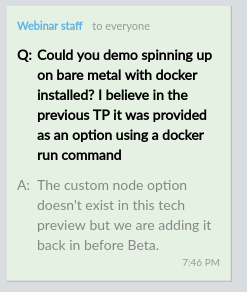
\includegraphics{assets/rancher-tp2-baremetal.png}\\

\hypertarget{uruchamianie-wersji-v2.0.0-alpha10}{%
\subsubsection{\texorpdfstring{Uruchamianie wersji
\texttt{v2.0.0-alpha10}}{Uruchamianie wersji v2.0.0-alpha10}}\label{uruchamianie-wersji-v2.0.0-alpha10}}

Testy przeprowadziłem na maszynach wirtualnych
\passthrough{\lstinline!VirtualBox!} w trybie bezdyskowym systemu
operacyjnego \passthrough{\lstinline!CoreOS!} z wykorzystaniem
repozytorium
\href{https://github.com/nazarewk/ipxe-boot}{\passthrough{\lstinline!ipxe-boot!}}.

Węzeł zarządzający uruchomiłem poniższą komendą:

\begin{lstlisting}[language=bash]
docker run --rm --name rancher -d -p 8080:8080 rancher/server:v2.0.0-alpha10
\end{lstlisting}

Pierwszym krokiem było zalogowanie się~do panelu administracyjnego
Ranchera dostępnego na porcie 8080 lokalnej maszyny i uzyskanie komendy
konfigurującej węzeł roboczy. Kolejnym i ostatnim krokiem konfiguracji
było uruchomienie uzyskanej komendy na dowolnej liczbie węzłów
roboczych:

\begin{lstlisting}[language=bash]
sudo docker run --rm --privileged \
  -v /var/run/docker.sock:/var/run/docker.sock \
  -v /var/lib/rancher:/var/lib/rancher \
  rancher/agent:v1.2.9 \
  http://192.168.56.1:8080/v1/scripts/B52944BEFAA613F0CE90:1514678400000:E2yB6KfxzSix4YHti39BTw5RbKw
\end{lstlisting}

W ciągu 2 godzin przeglądu nie udało mi się zautomatyzować procesu
uzyskiwania ww. komendy.

\hypertarget{napotkane-bux142ux119dy}{%
\paragraph{Napotkane błędy}\label{napotkane-bux142ux119dy}}

W wersji \passthrough{\lstinline!v2.0.0-alpha10!} losowo pojawia
się~błąd \href{https://github.com/rancher/rancher/issues/10396}{Upgrade
Environment}.

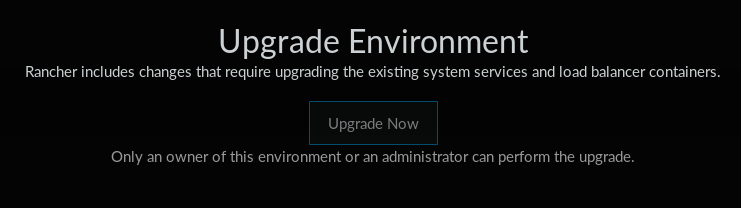
\includegraphics[width=5.20833in,height=1.45833in]{assets/rancher2-error.png}\\

\hypertarget{wnioski}{%
\subsubsection{Wnioski}\label{wnioski}}

Rancher na chwilę obecną (styczeń 2018 roku) jest bardzo wygodnym, ale
również niestabilnym rozwiązaniem. Ze tego względu odrzucam Ranchera
jako rozwiązanie problemu uruchamiania klastra
\passthrough{\lstinline!k8s!}.

\hypertarget{openshift-origin}{%
\section{OpenShift Origin}\label{openshift-origin}}

Według
\href{https://docs.openshift.org/latest/getting_started/administrators.html}{dokumentacji}
istnieją~dwie metody uruchamiania serwera, w Dockerze i bezpośrednio na
systemie Linux.

Zdecydowałem się~uruchomić~system w Dockerze ze względu na uniwersalność
rozwiązania. Komendą~uruchamiającą~serwer był:

\begin{lstlisting}[language=bash]
docker run -d --name "origin" \
  --privileged --pid=host --net=host \
  -v /:/rootfs:ro \
  -v /var/run:/var/run:rw \
  -v /sys:/sys \
  -v /sys/fs/cgroup:/sys/fs/cgroup:rw \
  -v /var/lib/docker:/var/lib/docker:rw \
  -v /var/lib/origin/openshift.local.volumes:/var/lib/origin/openshift.local.volumes:rslave \
  openshift/origin start --public-master
\end{lstlisting}

W porównaniu do przykładu z dokumentacji dodany został~argument
\passthrough{\lstinline!--public-master!} w celu uruchomienia interfejsu
graficznego.

\hypertarget{sterowniki-cgroup}{%
\subsubsection{\texorpdfstring{Sterowniki
\texttt{cgroup}}{Sterowniki cgroup}}\label{sterowniki-cgroup}}

Większość dystrybucji \passthrough{\lstinline!Linuxa!} (np. Arch,
CoreOS, Fedora, Debian) nie konfiguruje sterownika
\passthrough{\lstinline!cgroup!} Dockera i korzysta z domyślnego
\passthrough{\lstinline!cgroupfs!}, wersję~sterownika można zweryfikować
komendą~\passthrough{\lstinline!docker info | grep -i cgroup!}.

OpenShift korzysta ze sterownika \passthrough{\lstinline!systemd!}, a
\passthrough{\lstinline!kubelet!} w trakcie rozruchu weryfikuje
zgodność~sterowników, co skutkuje
\href{https://github.com/openshift/origin/issues/14766}{niekompatybilnością
z domyślną konfiguracją Dockera}, objawiającą się~poniższym błędem:

\begin{lstlisting}
F0120 19:18:58.708005   25376 node.go:269] failed to run Kubelet: failed to create kubelet: misconfiguration: kubelet cgroup driver: "systemd" is different from docker cgroup driver: "cgroupfs"
\end{lstlisting}

Problem można rozwiązać dodając argumenty
\passthrough{\lstinline!--exec-opt native.cgroupdriver=systemd!} do
komendy uruchamiającej główny proces Dockera.

\hypertarget{pruxf3ba-uruchomienia-serwera-na-systemie-arch-linux}{%
\subsubsection{Próba uruchomienia serwera na systemie Arch
Linux}\label{pruxf3ba-uruchomienia-serwera-na-systemie-arch-linux}}

Po rozwiązniu powyższego problemu i udanym uruchomieniu ww. komendy
rozruchowej przeszedłem do dalszych etapów instalacji zgodnie z
dokumentacją:

\begin{enumerate}
\def\labelenumi{\arabic{enumi}.}
\tightlist
\item
  Uruchomiłem linię komend OpenShift i zalogowałem się jako użytkownik
  testowy:
\end{enumerate}

\begin{lstlisting}
$ docker exec -it origin bash
\end{lstlisting}

\begin{lstlisting}
$ oc login
Username: test
Password: test
\end{lstlisting}

\begin{enumerate}
\def\labelenumi{\arabic{enumi}.}
\setcounter{enumi}{1}
\tightlist
\item
  Stworzyłem nowy projekt:
\end{enumerate}

\begin{lstlisting}
$ oc new-project test
\end{lstlisting}

\begin{enumerate}
\def\labelenumi{\arabic{enumi}.}
\setcounter{enumi}{2}
\tightlist
\item
  Pobrałem przykładową aplikację:
\end{enumerate}

\begin{lstlisting}
$ oc tag --source=docker openshift/deployment-example:v1 deployment-example:latest
\end{lstlisting}

\begin{enumerate}
\def\labelenumi{\arabic{enumi}.}
\setcounter{enumi}{3}
\tightlist
\item
  Uruchomiłem instancję aplikacji:
\end{enumerate}

\begin{lstlisting}
$ oc new-app deployment-example:latest
\end{lstlisting}

Uruchomienie przykładowej zakończyło się poniższym błędem:

\begin{lstlisting}
$ watch -n 5 oc status
In project test on server https://192.168.0.87:8443

svc/deployment-example - 172.30.52.184:8080
  dc/deployment-example deploys istag/deployment-example:latest 
    deployment #1 failed 1 minute ago: config change
\end{lstlisting}

Próba uruchomienia OpenShift Origin na Arch Linux zakończyła się
niepowodzeniem.

\hypertarget{pruxf3ba-uruchomienia-serwera-na-fedora-atomic-host-w-virtualbox}{%
\subsubsection{Próba uruchomienia serwera na Fedora Atomic Host w
VirtualBox}\label{pruxf3ba-uruchomienia-serwera-na-fedora-atomic-host-w-virtualbox}}

Następnie spróbowałem uruchomić OpenShift Origin na oficjalnie
wspieranym systemie operacyjnym
\passthrough{\lstinline!Fedora Atomic Host!} z użyciem Vagranta w
poniższej konfiguracji \passthrough{\lstinline!Vagrantfile!}:

\begin{lstlisting}[language=Ruby]
# -*- mode: ruby -*-
# vi: set ft=ruby :

Vagrant.configure("2") do |config|
  config.vm.box = "fedora/27-atomic-host"
  config.vm.box_check_update = false
  config.vm.network "forwarded_port", guest: 8443, host: 18443, host_ip: "127.0.0.1"
  config.vm.network "forwarded_port", guest: 8080, host: 18080, host_ip: "127.0.0.1"
  config.vm.provider "virtualbox" do |vb|
    vb.gui = false
    vb.memory = "8192"
  end
  config.vm.provision "shell", inline: <<-SHELL
  SHELL
end
\end{lstlisting}

Maszynę z lokalnym dyskiem uruchomiłem komendami
\passthrough{\lstinline!vagrant up!}, a następnie uzyskałem do niej
dostęp komendą~\passthrough{\lstinline!vagrant ssh!}. Kroki 1-4 były
analogiczne do uruchamiania na \passthrough{\lstinline!Arch Linux!}, po
czym przeszedłem do kolejnych kroków z dokumentacji:

\begin{enumerate}
\def\labelenumi{\arabic{enumi}.}
\setcounter{enumi}{4}
\tightlist
\item
  Odczekałem aż przykładowa aplikacja się uruchomi i zweryfikowałem jej
  działanie:
\end{enumerate}

\begin{lstlisting}
$ watch -n 5 oc status
In project test on server https://10.0.2.15:8443

svc/deployment-example - 172.30.221.105:8080
  dc/deployment-example deploys istag/deployment-example:latest 
    deployment #1 deployed 3 seconds ago - 1 pod
\end{lstlisting}

\begin{lstlisting}
$ curl http://172.30.221.105:8080 | grep v1
<div class="box"><h1>v1</h1><h2></h2></div>
\end{lstlisting}

\begin{enumerate}
\def\labelenumi{\arabic{enumi}.}
\setcounter{enumi}{5}
\tightlist
\item
  Przeprowadziłem aktualizację~aplikacji i ponownie zweryfikowałem jej
  działanie:
\end{enumerate}

\begin{lstlisting}
$ oc tag --source=docker openshift/deployment-example:v2 deployment-example:latest
Tag deployment-example:latest set to openshift/deployment-example:v2.
\end{lstlisting}

\begin{lstlisting}
$ watch -n 5 oc status
In project test on server https://10.0.2.15:8443

svc/deployment-example - 172.30.221.105:8080
  dc/deployment-example deploys istag/deployment-example:latest 
    deployment #2 running for 8 seconds - 1 pod
    deployment #1 deployed 8 minutes ago - 1 pod
\end{lstlisting}

\begin{lstlisting}
$ curl -s http://172.30.221.105:8080 | grep v2
<div class="box"><h1>v2</h1><h2></h2></div>
\end{lstlisting}

\begin{enumerate}
\def\labelenumi{\arabic{enumi}.}
\setcounter{enumi}{6}
\tightlist
\item
  Próba dostania się~do graficznego panelu administracyjnego zakończyła
  się niepowodzeniem:
\end{enumerate}

\begin{lstlisting}
$ curl -k 'https://localhost:8443/console/'
missing service (service "webconsole" not found)
missing route (service "webconsole" not found)
\end{lstlisting}

Nie znalazłem rozwiązania powyższego problemu w internecie, ani na
oficjalnym kanale \passthrough{\lstinline!#openshift!} na
\passthrough{\lstinline!irc.freenode.net!}.

\hypertarget{wnioski-1}{%
\subsubsection{Wnioski}\label{wnioski-1}}

Panel administracyjny klastra \passthrough{\lstinline!OpenShift Origin!}
jest jedyną~znaczącą przewagą nad \passthrough{\lstinline!kubespray!}.
Reszta zarządzania klastrem odbywa się również za pomocą repozytorium
skryptów Ansibla
(\href{https://docs.openshift.com/enterprise/3.0/admin_guide/manage_nodes.html\#adding-nodes}{w
tym dodawanie kolejnych węzłów klastra}).

Z powodu braku dostępu do ww. panelu próbę uruchomienia
\passthrough{\lstinline!OpenShift Origin!} uznaję za nieudaną i odrzucam
to narzędzie.

\hypertarget{kubespray-1}{%
\section{kubespray}\label{kubespray-1}}

Kroki podjęte w celu przetestowania narzędzia
\passthrough{\lstinline!kubespray!} zostały zawarte w skrypcie
\passthrough{\lstinline!bin/setup-cluster!} z repozytorium
\href{https://github.com/nazarewk/kubernetes-cluster}{kubernetes-cluster}.
Pełny kod źródłowy został zawarty w ``Dodatku B''.

W trakcie testowania narzędzia \passthrough{\lstinline!kubespray!} nie
napotkałem żadnych problemów, a szczegóły konfiguracji zawarłem jedynie
w kolejnych rozdziałach.

\hypertarget{wstux119pna-implementacja-kubespray-w-laboratorium-225}{%
\chapter{Wstępna implementacja kubespray w laboratorium
225}\label{wstux119pna-implementacja-kubespray-w-laboratorium-225}}

Po wybraniu narzędzia \passthrough{\lstinline!kubespray!} przystąpiłem
do jego uruchomienia w laboratorium 225 w celu dopracowania ostatecznej
konfiguracji.

Repozytorium \passthrough{\lstinline!kubernetes-cluster!} pobrałem do
folderu
\passthrough{\lstinline!/home/stud/nazarewk/kubernetes/kubernetes-cluster!}
na maszynie \passthrough{\lstinline!ldap!}.

Konieczne było przygotowanie dwóch plików konfigurujących rozruch
CoreOS.

\hypertarget{zetiswwwbootcoreos.ipxe}{%
\paragraph{\texorpdfstring{\texttt{zetis/WWW/boot/coreos.ipxe}}{zetis/WWW/boot/coreos.ipxe}}\label{zetiswwwbootcoreos.ipxe}}

jest plikiem konfiguracyjnym programu rozruchowego iPXE. Został
udostępniony pod adresem
\passthrough{\lstinline!http://vol/\~nazarewk/boot/coreos.ipxe!},
zawierał:

\begin{lstlisting}
#!ipxe
set http http://vol
set ftp http://ftp/pub/

set base-url ${ftp}/Linux/CoreOS/alpha
set ignition ${http}/~nazarewk/boot/coreos.ign

set opts ${opts} coreos.autologin
set opts ${opts} coreos.first_boot=1 coreos.config.url=${ignition}
set opts ${opts} systemd.journald.max_level_console=debug
kernel ${base-url}/coreos_production_pxe.vmlinuz ${opts}
initrd ${base-url}/coreos_production_pxe_image.cpio.gz

boot
\end{lstlisting}

\hypertarget{zetiswwwbootcoreos.yml}{%
\paragraph{\texorpdfstring{\texttt{zetis/WWW/boot/coreos.yml}}{zetis/WWW/boot/coreos.yml}}\label{zetiswwwbootcoreos.yml}}

jest plikiem Container Linux Config, z którego skryptem
\passthrough{\lstinline!bin/render-coreos!} generowany jest docelowy
plik konfiguracyjny Ignition
\passthrough{\lstinline!zetis/WWW/boot/coreos.ign!}.

Przykładem pliku \passthrough{\lstinline!coreos.yml!} tworzącego
użytkownika \passthrough{\lstinline!admin!} w grupach
\passthrough{\lstinline!docker!} i \passthrough{\lstinline!sudo!} oraz
dodającego klucz dostępowy SSH jest:

\begin{lstlisting}
passwd:
  users:
  - name: admin
    groups: [sudo, docker]
    ssh_authorized_keys:
    - ssh-rsa <klucz RSA> nazarewk
\end{lstlisting}

Na podstawie powyższego pliku skrypt
\passthrough{\lstinline!bin/render-coreos!} generuje następujący plik
\passthrough{\lstinline!coreos.ign!} w formacie JSON:

\begin{lstlisting}
{
  "ignition": {
    "config": {},
    "timeouts": {},
    "version": "2.1.0"
  },
  "networkd": {},
  "passwd": {
    "users": [
      {
        "groups": [
          "sudo",
          "docker"
        ],
        "name": "admin",
        "sshAuthorizedKeys": [
          "ssh-rsa <klucz RSA> nazarewk"
        ]
      }
    ]
  },
  "storage": {},
  "systemd": {}
}
\end{lstlisting}

Plik \passthrough{\lstinline!coreos.ign!} został udostępniony pod
adresem \passthrough{\lstinline!http://vol/\~nazarewk/boot/coreos.ign!}.

Po przygotowaniu powyższych plików konieczne było wskazanie ich maszynom
wywołując poniższą~komendę na maszynie \passthrough{\lstinline!volt!}:

\begin{lstlisting}[language=bash]
sudo lab 's4 s5 s6 s8 s9' boot http://vol/~nazarewk/boot/coreos.ipxe 
\end{lstlisting}

\hypertarget{konfiguracja-kubespray}{%
\section{Konfiguracja kubespray}\label{konfiguracja-kubespray}}

Konfiguracja \passthrough{\lstinline!kubespray!} ogranicza się~do
skopiowania przykładowego inwentarza i edycji plików
\passthrough{\lstinline!inventory.cfg!} oraz
\passthrough{\lstinline!group\_vars/all.yml!}.

\hypertarget{inventory.cfg}{%
\paragraph{\texorpdfstring{\texttt{inventory.cfg}}{inventory.cfg}}\label{inventory.cfg}}

jest plikiem INI reprezentującym topologię~klastra
\passthrough{\lstinline!k8s!}. Składa się~on z następujących sekcji:

\begin{itemize}
\tightlist
\item
  definicji~wszystkich węzłów klastra w sekcji
  \passthrough{\lstinline![all]!},
\item
  węzłów na których uruchomiony jest klaster
  \passthrough{\lstinline!etcd!} w sekcji
  \passthrough{\lstinline![etcd]!},
\item
  węzłów zarządzających w sekcji
  \passthrough{\lstinline![kube-master]!},
\item
  węzłów roboczych w sekcji \passthrough{\lstinline![kube-node]!},
\item
  połączenia sekcji \passthrough{\lstinline![kube-master]!} i
  \passthrough{\lstinline![kube-node]!} w
  sekcję~\passthrough{\lstinline![k8s-cluster]!}.
\end{itemize}

Kompletnym przykładem pliku dla laboratorium 225 jest:

\begin{lstlisting}
[all]
s4  ansible_host=s4 ip=10.146.225.4 ansible_python_interpreter=/opt/bin/python
s5  ansible_host=s5 ip=10.146.225.5 ansible_python_interpreter=/opt/bin/python
s6  ansible_host=s6 ip=10.146.225.6 ansible_python_interpreter=/opt/bin/python
;s8  ansible_host=s8 ip=10.146.225.8 ansible_python_interpreter=/opt/bin/python
;s9  ansible_host=s9 ip=10.146.225.9 ansible_python_interpreter=/opt/bin/python

[kube-master]
s4

[kube-node]
s5
s6 

[etcd]
s4

[k8s-cluster:children]
kube-node
kube-master
\end{lstlisting}

\hypertarget{group_varsall.yml}{%
\paragraph{\texorpdfstring{\texttt{group\_vars/all.yml}}{group\_vars/all.yml}}\label{group_varsall.yml}}

jest plikiem YAML zawierającym parametry wywołania
\passthrough{\lstinline!kubespray!} wspólne dla wszystkich węzłów.

Minimalną konfiguracją dla systemu \passthrough{\lstinline!CoreOS!}
jest:

\begin{lstlisting}
bootstrap_os: coreos  # automatyczna instalacja Pythona na CoreOS
kube_basic_auth: true  # podstawowe logowanie do Dashboardu Kubernetes
kubeconfig_localhost: true  # konfiguracja lokalnego kubectl
download_run_once: true  # pozwala na jednorazowe pobieranie plikow 
\end{lstlisting}

\hypertarget{napotkane-problemy}{%
\section{Napotkane problemy}\label{napotkane-problemy}}

\hypertarget{klonowanie-repozytoriuxf3w-bez-logowania}{%
\subsubsection{Klonowanie repozytoriów bez
logowania}\label{klonowanie-repozytoriuxf3w-bez-logowania}}

W celu umożliwienia anonimowego klonowania repozytorium z Githuba,
konieczne było wykorzystanie protokołu \passthrough{\lstinline!https!}
zamiast \passthrough{\lstinline!git!}:

\begin{lstlisting}
git clone https://github.com/nazarewk/kubernetes-cluster.git
\end{lstlisting}

Zmiana musiała być~wprowadzona również~do submodułów
\passthrough{\lstinline!git!}.

\hypertarget{zdejmowanie-atrybutu-wykonywalnoux15bci-pliku}{%
\subsubsection{Zdejmowanie atrybutu wykonywalności
pliku}\label{zdejmowanie-atrybutu-wykonywalnoux15bci-pliku}}

W konfiguracji uczelnianej \passthrough{\lstinline!git!} nie ustawia
zdejmuje atrybut wykonalności pobieranych plików. Po każdej komendzie
\passthrough{\lstinline!git pull!} konieczne było wywołanie komendy
\passthrough{\lstinline!chmod +x bin/*!}.

\hypertarget{konfiguracja-bezhasux142owego-dostux119pu-ssh}{%
\subsubsection{Konfiguracja bezhasłowego dostępu
SSH}\label{konfiguracja-bezhasux142owego-dostux119pu-ssh}}

W celu uruchomienia narzędzia \passthrough{\lstinline!kubespray!} w
trybie bezinterakcyjnym konieczna była konfiguracja bezhasłowego dostępu
SSH do zarządzanych maszyn. Powyższy problem rozwiązuje dodanie
poniższych wpisów w pliku \passthrough{\lstinline!\~/.ssh/config!}:

\begin{lstlisting}
Host s?
  User admin
  StrictHostKeyChecking no
  UserKnownHostsFile /dev/null
  IdentityFile ~/.ssh/id_rsa
  IdentitiesOnly yes
\end{lstlisting}

\hypertarget{problemy-z-sieciux105-uczelnianux105}{%
\subsubsection{Problemy z siecią
uczelnianą}\label{problemy-z-sieciux105-uczelnianux105}}

W trakcie pierwszego uruchamiania \passthrough{\lstinline!kubespray!}
występowały przeciążenia sieci uczelnianej, w związku z tym komendy były
tracone. Problemowi zaradzono konfigurując Ansible do powtarzania
nieudanych komend.

\hypertarget{ograniczenie-3-serweruxf3w-dns-w-kubespray}{%
\subsubsection{Ograniczenie 3 serwerów DNS w
kubespray}\label{ograniczenie-3-serweruxf3w-dns-w-kubespray}}

\passthrough{\lstinline!kubespray!} nie radzi sobie z więcej niż~trzema
wpisami DNS na konfigurowanych maszynach. Ograniczenie to objawiło się
na maszynie \passthrough{\lstinline!s8!}, która konfigurowała dodatkowy
interfejs sieciowy.

Problemu można uniknąć wyłączając zbędne interfejsy sieciowe.

\hypertarget{niewystarczajux105ca-iloux15bux107pamiux119ci-ram-na-maszynie-s2}{%
\subsubsection{Niewystarczająca ilość~pamięci RAM na maszynie
s2}\label{niewystarczajux105ca-iloux15bux107pamiux119ci-ram-na-maszynie-s2}}

Maszyna \passthrough{\lstinline!s2!} nie posiada ilości pamięci RAM
wystarczającej do uruchomienia węzła \passthrough{\lstinline!k8s!} i nie
powinna być wykorzystywana.

\hypertarget{eksperymentalna-konfiguracja-narzux119dzia-vault-w-kubespray}{%
\subsubsection{Eksperymentalna konfiguracja narzędzia Vault w
kubespray}\label{eksperymentalna-konfiguracja-narzux119dzia-vault-w-kubespray}}

W trakcie testów \passthrough{\lstinline!kubespray!} zostało rozszerzone
o wsparcie narzędzia \passthrough{\lstinline!Vault!} firmy HashiCorp.
Rozszerzenie okazało się niekompletne i konieczne było jego wyłączenie.

\hypertarget{logowanie-do-kubernetes-dashboard}{%
\subsubsection{Logowanie do Kubernetes
Dashboard}\label{logowanie-do-kubernetes-dashboard}}

Domyślna nazwa użytkownika Dashboardu to \passthrough{\lstinline!kube!},
a hasło znajduje się w pliku
\passthrough{\lstinline!credentials/kube\_user!}.

W starszej wersji \passthrough{\lstinline!k8s!} i/lub
\passthrough{\lstinline!kubespray!} brakowało opcji logowania przy
pomocy nazwy użytkownika i hasła:

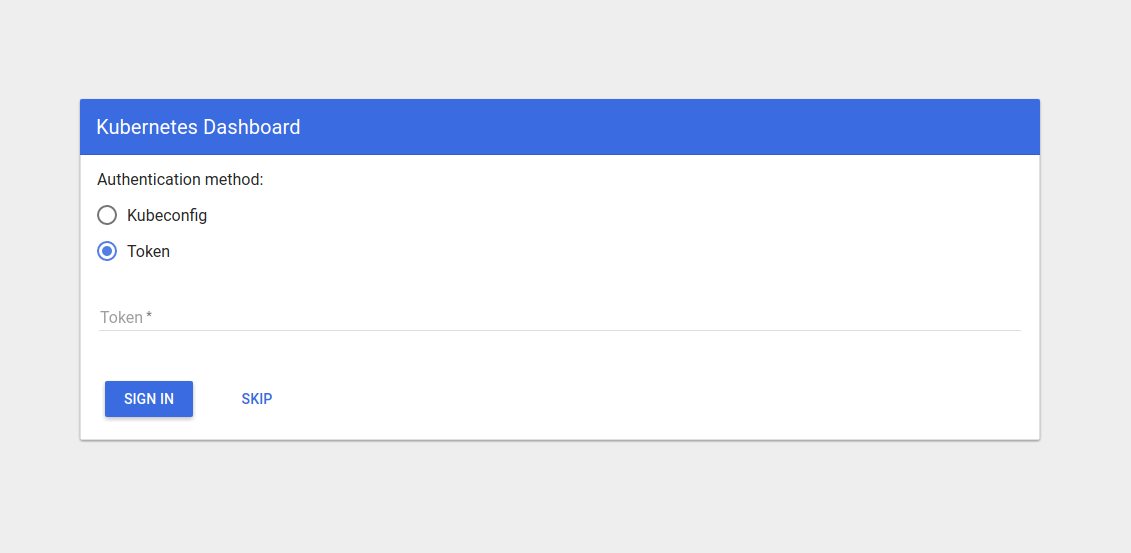
\includegraphics[width=5.20833in,height=2.5in]{assets/dashboard-login-old.png}\\

Od 29 stycznia 2018 roku zaobserwowany został poprawny ekran logowania
(opcja \passthrough{\lstinline!Basic!}):

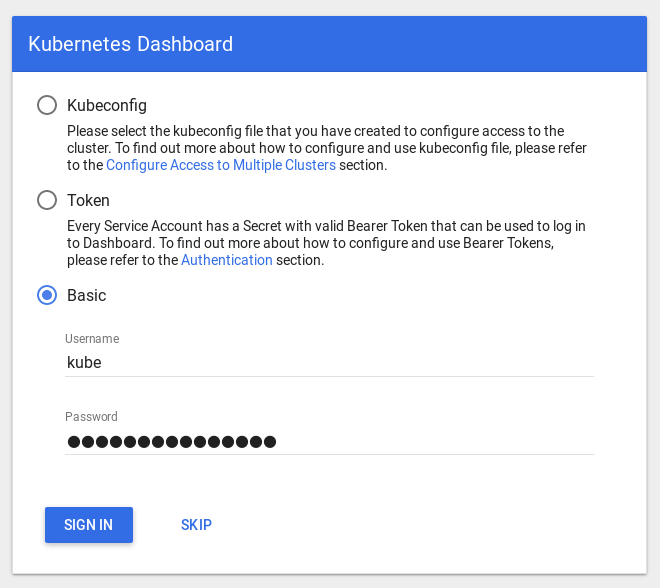
\includegraphics[width=5.20833in,height=4.63542in]{assets/dashboard-login-new.png}\\

\hypertarget{instalacja-dodatkowych-aplikacji-z-uux17cyciem-kubespray}{%
\subsubsection{Instalacja dodatkowych aplikacji z użyciem
kubespray}\label{instalacja-dodatkowych-aplikacji-z-uux17cyciem-kubespray}}

\passthrough{\lstinline!kubespray!} ma wbudowaną instalację kilku
dodatkowych aplikacji playbookiem
\passthrough{\lstinline!upgrade-cluster.yml!} z tagiem
\passthrough{\lstinline!apps!} (skrypt
\passthrough{\lstinline!bin/setup-cluster-upgrade!}). Ze względu na
liczne pojawiające się błędy temat został zarzucony.

\hypertarget{uruchomienie-helm}{%
\subsubsection{Uruchomienie Helm}\label{uruchomienie-helm}}

Instalacja menadżera pakietów sprowadza się~do:

\begin{enumerate}
\def\labelenumi{\arabic{enumi}.}
\tightlist
\item
  ściągnięcia pliku wykonywalnego \passthrough{\lstinline!helm!},
\item
  stworzenie roli RBAC dla serwerowego komponentu
  \passthrough{\lstinline!Tiller!},
\item
  Wywołanie komendy
  \passthrough{\lstinline!helm init --service-account tiller!}
\end{enumerate}

Wszystkie kroki zawierają się w skrypcie
\passthrough{\lstinline!bin/install-helm!}. Ze względu na braku
dystrybucji \passthrough{\lstinline!Helm!} na
\passthrough{\lstinline!FreeBSD!} całość jest uruchamiana przez SSH na
węźle zarządzającym (domyślnie \passthrough{\lstinline!s4!}).

Większość dostępnych~pakietów wymaga trwałych zasobów dyskowych, więc
temat nie był dalej zgłębiany.

\hypertarget{prezentacja-docelowej-konfiguracji-klastra-kubernetes-w-sieci-uczelnianej}{%
\chapter{Prezentacja docelowej konfiguracji klastra Kubernetes w sieci
uczelnianej}\label{prezentacja-docelowej-konfiguracji-klastra-kubernetes-w-sieci-uczelnianej}}

W tym rozdziale opisana jest pełna procedura uruchomienia klastra
\passthrough{\lstinline!Kubernetes!} z wykorzystaniem opracowanych
skryptów. Wywoływane komendy są w formacie
\passthrough{\lstinline!<nazwa\_hosta>\% <komenda>!}. Kolejnymi liniami
fragmentów kodu jest standardowe wyjście wywoływanych komend, a trzy
kropki \passthrough{\lstinline!...!} reprezentują~jego wycięte
fragmenty.

Pełną konfiguracja \passthrough{\lstinline!k8s!} można uruchomić z
maszyny \passthrough{\lstinline!ldap!}; znajduje się ona w folderze
\passthrough{\lstinline!/pub/Linux/CoreOS/zetis/kubernetes!}, który
zawiera następujące pliki i foldery:

\begin{itemize}
\tightlist
\item
  \passthrough{\lstinline!kubernetes-cluster!} - moje repozytorium
  zawierające konfigurację i skrypty pozwalające uruchomić klaster,
\item
  \passthrough{\lstinline!boot!} - skrót do folderu
  \passthrough{\lstinline!kubernetes-cluster/zetis/WWW/boot!}
  zawierającego konfigurację iPXE oraz Ignition:

  \begin{itemize}
  \tightlist
  \item
    \passthrough{\lstinline!coreos.ipxe!} - konfiguracja iPXE,
  \item
    \passthrough{\lstinline!coreos.ign!} - konfiguracja Ignition,
  \end{itemize}
\end{itemize}

\hypertarget{procedura-uruchomienia-klastra}{%
\section{Procedura uruchomienia
klastra}\label{procedura-uruchomienia-klastra}}

\begin{enumerate}
\def\labelenumi{\arabic{enumi}.}
\tightlist
\item
  Wejście na maszynę \passthrough{\lstinline!ldap!} do folderu
  \passthrough{\lstinline!/pub/Linux/CoreOS/zetis/kubernetes/kubernetes-cluster!},
\item
  Upewnienie się, że klucz dostępowy SSH jest obecny w
  \passthrough{\lstinline!boot/coreos.ign!},
\item
  Uruchomienie maszyn-węzłów wybierając z menu
  \passthrough{\lstinline!iPXE CoreOS!} -\textgreater{}
  \passthrough{\lstinline!k8s!} lub wybierając w narzędziu
  \passthrough{\lstinline!boot!} bezpośrednio
  \passthrough{\lstinline!coreos kub!},
\item
  Weryfikacja bezhasłowego dostępu do węzłów, minimalna konfiguracja
  \passthrough{\lstinline!\~/.ssh/config!} to:
\end{enumerate}

\begin{lstlisting}
Host s?
  User admin
  IdentityFile ~/.ssh/id_rsa
  IdentitiesOnly yes
  StrictHostKeyChecking no
  UserKnownHostsFile /dev/null
\end{lstlisting}

\begin{enumerate}
\def\labelenumi{\arabic{enumi}.}
\setcounter{enumi}{4}
\item
  W razie braku, utworzenie folderu
  \passthrough{\lstinline!kubespray/my\_inventory!} komendą
  \passthrough{\lstinline!cp -rav kubespray/inventory kubespray/my\_inventory!}
\item
  Upewnienie się, że uruchomione maszyny są obecne w odpowiednich
  sekcjach pliku \passthrough{\lstinline!inventory/inventory.cfg!},
  domyślna konfiguracja pozwala na uruchomienie klastra na maszynach
  \passthrough{\lstinline!s4!}, \passthrough{\lstinline!s5!} i
  \passthrough{\lstinline!s6!} z jednym węzłem zarządzającym
  \passthrough{\lstinline!s4!}:
\end{enumerate}

\begin{lstlisting}
[all]
;s3  ip=10.146.225.3
s4  ip=10.146.225.4
s5  ip=10.146.225.5
s6  ip=10.146.225.6
;s7  ip=10.146.225.7
;s8  ip=10.146.225.8
;s9  ip=10.146.225.9
;sa  ip=10.146.225.10
;sb  ip=10.146.225.11
;sc  ip=10.146.225.12

[kube-master]
s4

[kube-node]
s5
s6

[etcd]
s4

[k8s-cluster:children]
kube-node
kube-master
\end{lstlisting}

\begin{enumerate}
\def\labelenumi{\arabic{enumi}.}
\setcounter{enumi}{6}
\tightlist
\item
  Upewnienie się, że plik
  \passthrough{\lstinline!inventory/group\_vars/all.yml!} zawiera
  poprawną konfigurację, na przykład:
\end{enumerate}

\begin{lstlisting}
cluster_name: zetis-kubernetes
bootstrap_os: coreos
kube_basic_auth: true
kubeconfig_localhost: true
kubectl_localhost: true
download_run_once: true
\end{lstlisting}

\begin{enumerate}
\def\labelenumi{\arabic{enumi}.}
\setcounter{enumi}{7}
\tightlist
\item
  Konfiguracja klastra skryptem
  \passthrough{\lstinline!bin/setup-cluster!}. Po około 10 minutach
  skrypt powinien zakończyć się wpisami pokroju:
\end{enumerate}

\begin{lstlisting}
...
PLAY RECAP ********
localhost                  : ok=2    changed=0    unreachable=0    failed=0   
s4                         : ok=281  changed=94   unreachable=0    failed=0   
s5                         : ok=346  changed=80   unreachable=0    failed=0   
s6                         : ok=186  changed=54   unreachable=0    failed=0   
...
\end{lstlisting}

\begin{enumerate}
\def\labelenumi{\arabic{enumi}.}
\setcounter{enumi}{8}
\tightlist
\item
  Weryfikacja konfiguracji węzłów:
\end{enumerate}

\begin{lstlisting}[language=bash]
ldap% bin/kubectl get nodes
NAME      STATUS    ROLES     AGE       VERSION
s4        Ready     master    2m        v1.9.1_coreos.0
s5        Ready     node      2m        v1.9.1_coreos.0
s6        Ready     node      2m        v1.9.1_coreos.0
\end{lstlisting}

\hypertarget{procedury-korzystania-z-klastra-kubernetes}{%
\section{Procedury korzystania z klastra
Kubernetes}\label{procedury-korzystania-z-klastra-kubernetes}}

Aby dodać użytkownika wywołujemy skrypt
\passthrough{\lstinline!bin/students!} z pierwszym argumentem będącym
nazwą użytkownika i drugim \passthrough{\lstinline!create!}.

Wywołanie skryptu \passthrough{\lstinline!bin/students nazarewk create!}
jest równoważne uruchomieniu komendy
\passthrough{\lstinline!kubectl create -f nazarewk.yml!}, gdzie plik
\passthrough{\lstinline!nazarewk.yml!} to:

\begin{lstlisting}
apiVersion: v1
kind: Namespace
metadata:
  name: nazarewk
  labels:
    name: nazarewk
---
apiVersion: v1
kind: ServiceAccount
metadata:
  name: nazarewk
  namespace: nazarewk
---
kind: RoleBinding
apiVersion: rbac.authorization.k8s.io/v1
metadata:
  name: nazarewk-admin-binding
  namespace: nazarewk
roleRef:
  kind: ClusterRole
  name: admin
  apiGroup: rbac.authorization.k8s.io
subjects:
- kind: ServiceAccount
  name: nazarewk
\end{lstlisting}

Tworzone są następujące obiekty Kubernetes:

\begin{itemize}
\tightlist
\item
  przestrzeń nazw użytkownika,
\item
  konto serwisowe użytkownika,
\item
  przypisanie kontu serwisowemu roli \passthrough{\lstinline!admin!},
  która daje pełny dostęp do jego przestrzeni nazw.
\end{itemize}

\hypertarget{przykux142adowa-procedura-korzystania-z-klastra}{%
\subsubsection{Przykładowa procedura korzystania z
klastra}\label{przykux142adowa-procedura-korzystania-z-klastra}}

\begin{enumerate}
\def\labelenumi{\arabic{enumi}.}
\tightlist
\item
  Stworzenie konta użytkownika
\end{enumerate}

\begin{lstlisting}
ldap% bin/students nazarewk create
namespace "nazarewk" created
serviceaccount "nazarewk" created
rolebinding "nazarewk-admin-binding" created
Tokens:
eyJhb<SKROCONY_TOKEN>ahHfxU-TRw
\end{lstlisting}

\begin{lstlisting}
ldap% bin/students
NAME          STATUS    AGE
default       Active    3m
kube-public   Active    3m
kube-system   Active    3m
nazarewk      Active    16s
\end{lstlisting}

\begin{enumerate}
\def\labelenumi{\arabic{enumi}.}
\setcounter{enumi}{1}
\tightlist
\item
  Skopiowanie przepustki użytkownika na (przykładową) maszynę
  \passthrough{\lstinline!s2!} z działającym systemem operacyjnym
  Ubuntu:
\end{enumerate}

\begin{lstlisting}
  ldap% bin/student-tokens nazarewk | ssh nazarewk@s2 "cat > /tmp/token"
\end{lstlisting}

\begin{enumerate}
\def\labelenumi{\arabic{enumi}.}
\setcounter{enumi}{2}
\tightlist
\item
  Pobranie narzędzia \passthrough{\lstinline!kubectl!}:
\end{enumerate}

\begin{lstlisting}
s2% cd /tmp
s2% curl -LO https://storage.googleapis.com/kubernetes-release/release/$(curl -s https://storage.googleapis.com/kubernetes-release/release/stable.txt)/bin/linux/amd64/kubectl
s2% chmod +x kubectl
s2% sudo mv kubectl /usr/local/bin
s2% source <(kubectl completion zsh)
\end{lstlisting}

\begin{enumerate}
\def\labelenumi{\arabic{enumi}.}
\setcounter{enumi}{3}
\tightlist
\item
  Weryfikacja braku konfiguracji narzędzia:
\end{enumerate}

\begin{lstlisting}
s2% kubectl get nodes
The connection to the server localhost:8080 was refused - did you specify the right host or port?
\end{lstlisting}

\begin{enumerate}
\def\labelenumi{\arabic{enumi}.}
\setcounter{enumi}{4}
\tightlist
\item
  Konfiguracja \passthrough{\lstinline!kubectl!} w najprostszy możliwy
  sposób, czyli aliasem:
\end{enumerate}

\begin{lstlisting}
s2% alias kubectl='command kubectl -s "https://s4:6443" --insecure-skip-tls-verify=true --token="$(cat /tmp/token)" -n nazarewk'
\end{lstlisting}

\begin{enumerate}
\def\labelenumi{\arabic{enumi}.}
\setcounter{enumi}{5}
\tightlist
\item
  Weryfikacja braku dostępu do zasobów globalnych klastra:
\end{enumerate}

\begin{lstlisting}
s2% kubectl get nodes
Error from server (Forbidden): nodes is forbidden: User "system:serviceaccount:nazarewk:nazarewk" cannot list nodes at the cluster scope
\end{lstlisting}

\begin{enumerate}
\def\labelenumi{\arabic{enumi}.}
\setcounter{enumi}{6}
\tightlist
\item
  Stworzenie \passthrough{\lstinline!Deployment!} przykładowej
  aplikacji:
\end{enumerate}

\begin{lstlisting}
s2% kubectl run echoserver --image=gcr.io/google_containers/echoserver:1.4 --port=8080 --replicas=2
deployment "echoserver" created
\end{lstlisting}

\begin{lstlisting}
s2% kubectl get deployments
NAME         DESIRED   CURRENT   UP-TO-DATE   AVAILABLE   AGE
echoserver   2         2         2            2           3m
\end{lstlisting}

\begin{lstlisting}
s2% kubectl get pods
NAME                         READY     STATUS    RESTARTS   AGE
echoserver-7b9bbf6ff-22df4   1/1       Running   0          4m
echoserver-7b9bbf6ff-c6kbv   1/1       Running   0          4m
\end{lstlisting}

\begin{enumerate}
\def\labelenumi{\arabic{enumi}.}
\setcounter{enumi}{7}
\tightlist
\item
  Stworzenie serwisu typu \passthrough{\lstinline!NodePort!} w celu
  dostępu do aplikacji:
\end{enumerate}

\begin{lstlisting}
s2% kubectl expose deployment echoserver --type=NodePort
service "echoserver" exposed
\end{lstlisting}

\begin{lstlisting}
s2% kubectl describe services/echoserver | grep -e NodePort:
NodePort:                 <unset>  30100/TCP
\end{lstlisting}

Wynik ostatniej komendy oznacza dostęp do aplikacji przez port
\passthrough{\lstinline!30100!} dowolnego węzła klastra.

\begin{enumerate}
\def\labelenumi{\arabic{enumi}.}
\setcounter{enumi}{8}
\tightlist
\item
  Weryfikacja działania aplikacji:
\end{enumerate}

\begin{lstlisting}
s2% curl s4:30100
CLIENT VALUES:
client_address=10.233.107.64
command=GET
real path=/
query=nil
request_version=1.1
request_uri=http://s4:8080/

SERVER VALUES:
server_version=nginx: 1.10.0 - lua: 10001

HEADERS RECEIVED:
accept=*/*
host=s4:30100
user-agent=curl/7.47.0
BODY:
-no body in request-
\end{lstlisting}

\begin{enumerate}
\def\labelenumi{\arabic{enumi}.}
\setcounter{enumi}{9}
\tightlist
\item
  Weryfikacja dostępu do aplikacji z maszyny
  \passthrough{\lstinline!ldap!}:
\end{enumerate}

\begin{lstlisting}
ldap% curl s4:30100
CLIENT VALUES:
client_address=10.233.107.64
command=GET
real path=/
query=nil
request_version=1.1
request_uri=http://s4:8080/

SERVER VALUES:
server_version=nginx: 1.10.0 - lua: 10001

HEADERS RECEIVED:
accept=*/*
host=s4:30100
user-agent=curl/7.58.0
BODY:
-no body in request-
\end{lstlisting}

\begin{enumerate}
\def\labelenumi{\arabic{enumi}.}
\setcounter{enumi}{10}
\tightlist
\item
  Usunięcie użytkownika:
\end{enumerate}

\begin{lstlisting}
ldap% bin/students nazarewk delete
namespace "nazarewk" deleted
serviceaccount "nazarewk" deleted
rolebinding "nazarewk-admin-binding" deleted
Tokens:
Error from server (NotFound): serviceaccounts "nazarewk" not found
\end{lstlisting}

\begin{enumerate}
\def\labelenumi{\arabic{enumi}.}
\setcounter{enumi}{11}
\tightlist
\item
  Weryfikacja usunięcia wszystkich zasobów użytkownika:
\end{enumerate}

\begin{lstlisting}
ldap% curl s4:30100
curl: (7) Failed to connect to s4 port 30100: Connection refused
\end{lstlisting}

\begin{lstlisting}
ldap% bin/kubectl get namespace 
NAME          STATUS    AGE
default       Active    46m
kube-public   Active    46m
kube-system   Active    46m
\end{lstlisting}

\hypertarget{podsumowanie}{%
\chapter{Podsumowanie}\label{podsumowanie}}

W niniejszej pracy omówiono zagadnienie konfiguracji klastra
\passthrough{\lstinline!Kubernetes!}. Przedstawione zostały elementarne
pojęcia z zakresu konfiguracji i korzystania z klastra
\passthrough{\lstinline!k8s!} bazowanego na maszynach bezdyskowych.
Bezpośrednim rezultatem pracy są skrypty implementujące klaster w sieci
uczelnianej oraz umożliwiające prowadzenie zajęć demonstracyjnych ze
studentami.

W związku z aktywnym rozwojem projektu \passthrough{\lstinline!k8s!}
stworzenie publikacji wyczerpującej temat nie jest możliwe. Wiele
obiecujących narzędzi pojawiało się i znacznie zmieniało w trakcie
pisania niniejszej pracy. Nie zostały one należycie opisane lub nie
nadawały się jeszcze do użytku w momencie jej zakończenia. Projekty te
mogłyby realizować~alternatywne implementacje poruszonych w tej pracy
zagadnień.

Ze względu na ograniczenia czasowe praca nie poruszyła zaawansowanych
zagadnień \passthrough{\lstinline!k8s!} oraz nie zaimplementowała
żadnych mechanizmów bazujących na zewnętrznych usługach. Przykładami
zagadnień, które mogłyby zostać w przyszłości opisane, są:

\begin{itemize}
\tightlist
\item
  integracja z sieciowymi systemami plików w celu utrwalenia danych,
\item
  bezobsługowe dołączanie nowych węzłów do klastra
  \passthrough{\lstinline!k8s!} działającego w sieci uczelnianiej,
\item
  opracowanie zajęć laboratoryjnych bazowanych na
  \passthrough{\lstinline!Kubernetes!}.
\end{itemize}

Przedstawiony we wstępie cel został osiągnięty, a wysiłek włożony w
realizację pracy zaowocował znacznym zwiększeniem kompetencji autora
związanych z tematyką konteneryzacji i
\passthrough{\lstinline!Kubernetes!}. Zdobyta wiedza jest bezcenną
wartością na rynku pracy.

\appendix

\hypertarget{wykaz-odnoux15bnikuxf3w}{%
\chapter{Wykaz odnośników}\label{wykaz-odnoux15bnikuxf3w}}

\theendnotes

\hypertarget{wykaz-kodu-ux17aruxf3dux142owego}{%
\chapter{Wykaz kodu źródłowego}\label{wykaz-kodu-ux17aruxf3dux142owego}}

\hypertarget{repozytorium-kubernetes-cluster}{%
\section{repozytorium
kubernetes-cluster}\label{repozytorium-kubernetes-cluster}}

\passthrough{\lstinline!kubernetes-cluster!}
(\passthrough{\lstinline!https://github.com/nazarewk/kubernetes-cluster!})
jest repozytorium Git, które zawiera kompletny kod źródłowy
wykorzystywany w tej pracy inżynierskiej.

Kod można znaleźć~i uruchomić w sieci uczelnianej z katalogu
\passthrough{\lstinline!/pub/Linux/CoreOS/zetis/kubernetes/kubernetes-cluster/!}
na maszynie \passthrough{\lstinline!ldap!}.

\hypertarget{binpull}{%
\subsubsection{bin/pull}\label{binpull}}

Pobiera aktualną wersję~repozytorium wraz z najnowszą wersją zależności:

\begin{lstlisting}[language=bash]
#!/bin/sh
# Author: Krzysztof Nazarewski <nazarewk@gmail.com>
# Purpose: git pull wrapper including submodule updates

git pull || (git fetch --all && git reset --hard origin)
git submodule update --init --remote --recursive
chmod +x ${0%/*}/*
\end{lstlisting}

\hypertarget{binvars}{%
\subsubsection{bin/vars}\label{binvars}}

Zawiera wspólne zmienne środowiskowe wykorzystywane w reszcie skryptów
oraz linii komend:

\begin{lstlisting}[language=bash]
#!/bin/sh
# Author: Krzysztof Nazarewski <nazarewk@gmail.com>
# Purpose: Holds common variables used in all other scripts

if [ -z "$KC_CONFIGURED" ]; then
  KC_CONFIGURED=1

  BIN="$(realpath ${0%/*})"
  PATH="$BIN:$PATH"
  PDIR="${BIN%/*}"
  VENV="$PDIR/.env"
  KUBESPRAY="$PDIR/kubespray"
  INVENTORY="$KUBESPRAY/my_inventory"
  CONFIG_FILE="$INVENTORY/inventory.cfg"

  export KUBECONFIG="$KUBESPRAY/artifacts/admin.conf"
  export ANSIBLE_CONFIG="$PDIR/ansible.cfg"
fi
\end{lstlisting}

\hypertarget{binensure-virtualenv}{%
\subsubsection{bin/ensure-virtualenv}\label{binensure-virtualenv}}

Konfiguruje środowisko Pythona, wraz z próbą instalacji brakującego
\passthrough{\lstinline!virtualenv!} przez
\passthrough{\lstinline!apt!}:

\begin{lstlisting}[language=bash]
#!/bin/sh
# Author: Krzysztof Nazarewski <nazarewk@gmail.com>
# Purpose: installs python virtualenv

. ${0%/*}/vars
python="$(which python)"
activate="$VENV/bin/activate"

find_virtualenv() {
    which virtualenv 2> /dev/null || which virtualenv
}

install_virtualenv () {
  # Installs pip and/or virtualenv

  local pip=$(which pip)
  local apt=$(which apt)
  if [ ! -z "$pip" ]; then
    sudo $pip install virtualenv
    return 0
  elif [ ! -z "$apt" ]; then
    sudo $apt install virtualenv
    return 0
  else
    echo 'Virtualenv, pip and apt-get are both missing, cannot proceed'
    exit 1
  fi
}

create_env () {
    local cmd=$(find_virtualenv)
    [ -z "$cmd" ] && install_virtualenv && cmd=$(find_virtualenv)

    $cmd -p $python $VENV
    . $activate

    pip install -U pip setuptools
}

[ -z "$python" ] && echo 'python is missing' && exit 1
[ -e "$activate" ] && . $activate || create_env
pip install -U -r $PDIR/requirements.txt
\end{lstlisting}

\hypertarget{binensure-configuration}{%
\subsubsection{bin/ensure-configuration}\label{binensure-configuration}}

Generuje brakujące pliki konfiguracyjne SSH,
\passthrough{\lstinline!inventory.cfg!} i
\passthrough{\lstinline!group\_vars/all.yml!} nie nadpisując
istniejących:

\begin{lstlisting}[language=bash]
#!/bin/sh
# Author: Krzysztof Nazarewski <nazarewk@gmail.com>
# Purpose: configures cluster (SSH, inventory, group_vars)

. ${0%/*}/vars
SSH_CFG_DST="$HOME/.ssh/config"
SSH_CFG="$PDIR/zetis/.ssh/kubernetes.conf"


is_ssh_config_missing () {
  cat << EOF | python
import sys
expected = open('$SSH_CFG', 'rb').read()
existing = open('$SSH_CFG_DST', 'rb').read()
sys.exit(expected in existing)
EOF
  return $?
}

is_ssh_config_missing && cat $SSH_CFG >> $SSH_CFG_DST

file="$INVENTORY/inventory.cfg"
[ -f "$file" ] || cat << EOF > "$file"
[all]
;s3  ip=10.146.225.3
s4  ip=10.146.225.4
s5  ip=10.146.225.5
s6  ip=10.146.225.6
;s7  ip=10.146.225.7
;s8  ip=10.146.225.8
;s9  ip=10.146.225.9
;sa  ip=10.146.225.10
;sb  ip=10.146.225.11
;sc  ip=10.146.225.12

[kube-master]
s4

[kube-node]
s5
s6

[etcd]
s4

[k8s-cluster:children]
kube-node
kube-master
EOF

file="$INVENTORY/group_vars/all.yml"
[ -f "$file" ] || cat << EOF > "$file"
cluster_name: zetis-kubernetes
bootstrap_os: coreos
kube_basic_auth: true
kubeconfig_localhost: true
kubectl_localhost: true
download_run_once: true
EOF
\end{lstlisting}

\hypertarget{binrender-coreos}{%
\subsubsection{bin/render-coreos}\label{binrender-coreos}}

Generuje konfigurację Ignition (JSON) na podstawie Container Linux
Config (YAML):

\begin{lstlisting}[language=bash]
#!/bin/sh
# Author: Krzysztof Nazarewski <nazarewk@gmail.com>
# Purpose: renders CoreOS Ignition (incl. retrieving binary)

. ${0%/*}/vars
ct_version=${1:-0.6.1}
boot="$PDIR/zetis/WWW/boot"
url='https://github.com/coreos/container-linux-config-transpiler'
url="$url/releases/download"
url="$url/v${ct_version}/ct-v${ct_version}-x86_64-unknown-linux-gnu"

wget -nc $url -O $BIN/ct
chmod +x $BIN/ct
$BIN/ct -pretty \
  -in-file "$boot/coreos.yml" \
  -out-file "$boot/coreos.ign"
\end{lstlisting}

\hypertarget{binsetup-cluster}{%
\subsubsection{bin/setup-cluster}\label{binsetup-cluster}}

Właściwy skrypt konfigurujący klaster na działających maszynach CoreOS:

\begin{lstlisting}[language=bash]
#!/bin/sh
# Author: Krzysztof Nazarewski <nazarewk@gmail.com>
# Purpose: sets up the cluster

. ${0%/*}/vars
. $BIN/ensure-configuration
. $BIN/activate

(
  cd $KUBESPRAY;
  ansible-playbook -i $INVENTORY/inventory.cfg cluster.yml -b -v $@
)

chmod -R 700 $KUBESPRAY/artifacts/admin.conf $KUBESPRAY/credentials

cat << EOF
Login credentials:
  user: kube
  password: $(cat $PDIR/credentials/kube_user)
EOF
\end{lstlisting}

\hypertarget{binsetup-cluster-full}{%
\subsubsection{bin/setup-cluster-full}\label{binsetup-cluster-full}}

Skrót do pobierania najnowszej wersji, a następnie uruchamiania klastra:

\begin{lstlisting}[language=bash]
#!/bin/sh
. ${0%/*}/vars

$BIN/pull
$BIN/setup-cluster $@
\end{lstlisting}

\hypertarget{binsetup-cluster-upgrade}{%
\subsubsection{bin/setup-cluster-upgrade}\label{binsetup-cluster-upgrade}}

Skrypt analogiczny do \passthrough{\lstinline!setup-cluster!}, ale
wywołujący \passthrough{\lstinline!upgrade-cluster.yml!} zamiast
\passthrough{\lstinline!cluster.yml!}:

\begin{lstlisting}[language=bash]
#!/bin/sh
# Author: Krzysztof Nazarewski <nazarewk@gmail.com>
# Purpose: runs upgrade-cluster.yml instead of cluster.yml

. ${0%/*}/vars
. $BIN/ensure-configuration
. $BIN/activate

cd $KUBESPRAY
ansible-playbook -i $INVENTORY/inventory.cfg upgrade-cluster.yml -b -v $@
\end{lstlisting}

\hypertarget{binkubectl}{%
\subsubsection{bin/kubectl}\label{binkubectl}}

Skrót \passthrough{\lstinline!kubectl!} z automatycznym dołączaniem
konfiguracji \passthrough{\lstinline!kubespray!}:

\begin{lstlisting}[language=bash]
#!/bin/sh
# Author: Krzysztof Nazarewski <nazarewk@gmail.com>
# Purpose: kubectl wrapper which uses generated  configurations

# Handle running kubectl from PATH
[ "${0%/*}" == "$0" ] && _bin=$(dirname $(which kubectl)) || _bin=${0%/*}
. $_bin/vars

local_bin="$PDIR/artifacts/kubectl"

if [ -f $local_bin ]; then
  chmod +x $local_bin
  kubectl=$local_bin
else
  kubectl=/usr/bin/kubectl
fi

$kubectl $@
\end{lstlisting}

\hypertarget{binstudents}{%
\subsubsection{bin/students}\label{binstudents}}

Skrypt zarządzający obiektami \passthrough{\lstinline!k8s!}
użytkowników, czyli studentów:

\begin{lstlisting}[language=bash]
#!/bin/sh
# Author: Krzysztof Nazarewski <nazarewk@gmail.com>
# Purpose: executes operations on users (create, get, describe, delete)

. ${0%/*}/vars

kubectl_command () {
local users="$1"
local cmd="$2"
for name in $users; do
  cat  <<EOF | $BIN/kubectl $cmd -f -
apiVersion: v1
kind: Namespace
metadata:
  name: ${name}
  labels:
    name: ${name}

---

apiVersion: v1
kind: ServiceAccount
metadata:
  name: ${name}
  namespace: ${name}

---

kind: RoleBinding
apiVersion: rbac.authorization.k8s.io/v1
metadata:
  name: ${name}-admin-binding
  namespace: ${name}
roleRef:
  kind: ClusterRole
  name: admin
  apiGroup: rbac.authorization.k8s.io
subjects:
- kind: ServiceAccount
  name: ${name}
EOF
  echo Tokens:
  $BIN/student-tokens ${name}
done
}

case $1 in
  ""|list)
    $BIN/kubectl get namespace
    ;;
  -h)
    cat << EOF
    Usage: $0 "<usernames>" create|get|describe|delete
      where <usernames> is a single-argument list of usernames
    You can also call it without arguments to list users (namespaces)
EOF
    ;;
  *)
    kubectl_command "$@"
    ;;
esac
\end{lstlisting}

\hypertarget{binstudent-tokens}{%
\subsubsection{bin/student-tokens}\label{binstudent-tokens}}

Listuje przepustki konkretnego użytkownika:

\begin{lstlisting}[language=bash]
#!/bin/sh
# Author: Krzysztof Nazarewski <nazarewk@gmail.com>
# Purpose: lists kubernetes authentication tokens for specified user

. ${0%/*}/vars
name=$1
args="--namespace $name get serviceaccount $name"
args="$args -o jsonpath={.secrets[*].name}"
for token in `$BIN/kubectl $args`; do
    args="get secrets $token --namespace $name"
    args="$args  -o jsonpath={.data.token}"
    $BIN/kubectl $args | base64 --decode
    echo
done
\end{lstlisting}

\hypertarget{bininstall-helm}{%
\subsubsection{bin/install-helm}\label{bininstall-helm}}

Instaluje menadżer pakietów \passthrough{\lstinline!Helm!}:

\begin{lstlisting}[language=bash]
#!/bin/sh
# Author: Krzysztof Nazarewski <nazarewk@gmail.com>
# Purpose: installs helm package manager into Kubernetes cluster

. ${0%/*}/vars

host=${1:-s4}

ssh () {
  command ssh $host sudo $@
}

cat <<EOF | ssh bash
export HELM_INSTALL_DIR=/opt/bin
url='https://raw.githubusercontent.com/kubernetes/helm/master/scripts/get'
[ -f /opt/bin/helm ] || curl \$url | bash
EOF

cat <<EOF | ssh kubectl create -f -
apiVersion: v1
kind: ServiceAccount
metadata:
  name: tiller
  namespace: kube-system
---
apiVersion: rbac.authorization.k8s.io/v1beta1
kind: ClusterRoleBinding
metadata:
  name: tiller
roleRef:
  apiGroup: rbac.authorization.k8s.io
  kind: ClusterRole
  name: cluster-admin
subjects:
  - kind: ServiceAccount
    name: tiller
    namespace: kube-system
EOF

ssh helm version | grep Server: || ssh helm init --service-account tiller
\end{lstlisting}

\hypertarget{zetis.sshkubernetes.conf}{%
\subsubsection{zetis/.ssh/kubernetes.conf}\label{zetis.sshkubernetes.conf}}

Częściowy plik konfiguracyjny SSH do umieszczenia w
\passthrough{\lstinline!\~/.ssh/config!}:

\begin{lstlisting}[language=bash]
Host s?
  User admin
  IdentityFile ~/.ssh/id_rsa
  IdentitiesOnly yes
  StrictHostKeyChecking no
  UserKnownHostsFile /dev/null
\end{lstlisting}

\hypertarget{zetiswwwbootcoreos.ipxe-1}{%
\subsubsection{zetis/WWW/boot/coreos.ipxe}\label{zetiswwwbootcoreos.ipxe-1}}

Skrypt iPXE uruchamiający maszynę z CoreOS:

\begin{lstlisting}[language=bash]
#!ipxe
set ftp http://ftp/pub/

set base-url ${ftp}/Linux/CoreOS/alpha
set ignition ${ftp}/Linux/CoreOS/zetis/kubernetes/boot/coreos.ign

set opts ${opts} coreos.autologin
set opts ${opts} coreos.first_boot=1 coreos.config.url=${ignition}
set opts ${opts} systemd.journald.max_level_console=debug
kernel ${base-url}/coreos_production_pxe.vmlinuz ${opts}
initrd ${base-url}/coreos_production_pxe_image.cpio.gz

boot
\end{lstlisting}

\hypertarget{zetiswwwbootcoreos.yml-1}{%
\subsubsection{zetis/WWW/boot/coreos.yml}\label{zetiswwwbootcoreos.yml-1}}

Plik konfiguracyjny Container Linux Config w formacie YAML, docelowo do
przepuszczenia przez narzędzie \passthrough{\lstinline!ct!}. Wyjątkowo
skróciłem ten skrypt, ze względu na długość kluczy SSH:

\begin{lstlisting}
passwd:
  users:
  - name: admin
    groups: [sudo, docker]
    ssh_authorized_keys:
    - ssh-rsa <klucz RSA> ato@volt.iem.pw.edu.pl
    - ssh-rsa <klucz RSA> nazarewk
    - ssh-rsa <klucz RSA> nazarewk@ldap.iem.pw.edu.pl
\end{lstlisting}

\hypertarget{zetiswwwbootcoreos.ign}{%
\subsubsection{zetis/WWW/boot/coreos.ign}\label{zetiswwwbootcoreos.ign}}

Z powyższego pliku wygenerowany zostaje (również skrócony) plik JSON:

\begin{lstlisting}
{
  "ignition": {
    "config": {},
    "timeouts": {},
    "version": "2.1.0"
  },
  "networkd": {},
  "passwd": {
    "users": [
      {
        "groups": [
          "sudo",
          "docker"
        ],
        "name": "admin",
        "sshAuthorizedKeys": [
          "ssh-rsa <klucz RSA> nazarewk",
          "ssh-rsa <klucz RSA> nazarewk@ldap.iem.pw.edu.pl",
          "ssh-rsa <klucz RSA> ato@volt.iem.pw.edu.pl"
        ]
      }
    ]
  },
  "storage": {},
  "systemd": {}
}
\end{lstlisting}

\hypertarget{repozytorium-ipxe-boot}{%
\section{repozytorium ipxe-boot}\label{repozytorium-ipxe-boot}}

\passthrough{\lstinline!ipxe-boot!}
(\passthrough{\lstinline!https://github.com/nazarewk/ipxe-boot!}) jest
repozytorium kodu umożliwiającego uruchomienie środowiska bezdyskowego
poza uczelnią.

Repozytorium nie zostało wykorzystane w finalnej konfiguracji, więc nie
będę opisywał jego zawartości.
\cleardoublepage
\end{document}
